% Options for packages loaded elsewhere
\PassOptionsToPackage{unicode}{hyperref}
\PassOptionsToPackage{hyphens}{url}
%
\documentclass[
]{book}
\usepackage{lmodern}
\usepackage{amssymb,amsmath}
\usepackage{ifxetex,ifluatex}
\ifnum 0\ifxetex 1\fi\ifluatex 1\fi=0 % if pdftex
  \usepackage[T1]{fontenc}
  \usepackage[utf8]{inputenc}
  \usepackage{textcomp} % provide euro and other symbols
\else % if luatex or xetex
  \usepackage{unicode-math}
  \defaultfontfeatures{Scale=MatchLowercase}
  \defaultfontfeatures[\rmfamily]{Ligatures=TeX,Scale=1}
\fi
% Use upquote if available, for straight quotes in verbatim environments
\IfFileExists{upquote.sty}{\usepackage{upquote}}{}
\IfFileExists{microtype.sty}{% use microtype if available
  \usepackage[]{microtype}
  \UseMicrotypeSet[protrusion]{basicmath} % disable protrusion for tt fonts
}{}
\makeatletter
\@ifundefined{KOMAClassName}{% if non-KOMA class
  \IfFileExists{parskip.sty}{%
    \usepackage{parskip}
  }{% else
    \setlength{\parindent}{0pt}
    \setlength{\parskip}{6pt plus 2pt minus 1pt}}
}{% if KOMA class
  \KOMAoptions{parskip=half}}
\makeatother
\usepackage{xcolor}
\IfFileExists{xurl.sty}{\usepackage{xurl}}{} % add URL line breaks if available
\IfFileExists{bookmark.sty}{\usepackage{bookmark}}{\usepackage{hyperref}}
\hypersetup{
  pdftitle={Meta-Workflow},
  pdfauthor={Miao YU},
  hidelinks,
  pdfcreator={LaTeX via pandoc}}
\urlstyle{same} % disable monospaced font for URLs
\usepackage{color}
\usepackage{fancyvrb}
\newcommand{\VerbBar}{|}
\newcommand{\VERB}{\Verb[commandchars=\\\{\}]}
\DefineVerbatimEnvironment{Highlighting}{Verbatim}{commandchars=\\\{\}}
% Add ',fontsize=\small' for more characters per line
\usepackage{framed}
\definecolor{shadecolor}{RGB}{248,248,248}
\newenvironment{Shaded}{\begin{snugshade}}{\end{snugshade}}
\newcommand{\AlertTok}[1]{\textcolor[rgb]{0.94,0.16,0.16}{#1}}
\newcommand{\AnnotationTok}[1]{\textcolor[rgb]{0.56,0.35,0.01}{\textbf{\textit{#1}}}}
\newcommand{\AttributeTok}[1]{\textcolor[rgb]{0.77,0.63,0.00}{#1}}
\newcommand{\BaseNTok}[1]{\textcolor[rgb]{0.00,0.00,0.81}{#1}}
\newcommand{\BuiltInTok}[1]{#1}
\newcommand{\CharTok}[1]{\textcolor[rgb]{0.31,0.60,0.02}{#1}}
\newcommand{\CommentTok}[1]{\textcolor[rgb]{0.56,0.35,0.01}{\textit{#1}}}
\newcommand{\CommentVarTok}[1]{\textcolor[rgb]{0.56,0.35,0.01}{\textbf{\textit{#1}}}}
\newcommand{\ConstantTok}[1]{\textcolor[rgb]{0.00,0.00,0.00}{#1}}
\newcommand{\ControlFlowTok}[1]{\textcolor[rgb]{0.13,0.29,0.53}{\textbf{#1}}}
\newcommand{\DataTypeTok}[1]{\textcolor[rgb]{0.13,0.29,0.53}{#1}}
\newcommand{\DecValTok}[1]{\textcolor[rgb]{0.00,0.00,0.81}{#1}}
\newcommand{\DocumentationTok}[1]{\textcolor[rgb]{0.56,0.35,0.01}{\textbf{\textit{#1}}}}
\newcommand{\ErrorTok}[1]{\textcolor[rgb]{0.64,0.00,0.00}{\textbf{#1}}}
\newcommand{\ExtensionTok}[1]{#1}
\newcommand{\FloatTok}[1]{\textcolor[rgb]{0.00,0.00,0.81}{#1}}
\newcommand{\FunctionTok}[1]{\textcolor[rgb]{0.00,0.00,0.00}{#1}}
\newcommand{\ImportTok}[1]{#1}
\newcommand{\InformationTok}[1]{\textcolor[rgb]{0.56,0.35,0.01}{\textbf{\textit{#1}}}}
\newcommand{\KeywordTok}[1]{\textcolor[rgb]{0.13,0.29,0.53}{\textbf{#1}}}
\newcommand{\NormalTok}[1]{#1}
\newcommand{\OperatorTok}[1]{\textcolor[rgb]{0.81,0.36,0.00}{\textbf{#1}}}
\newcommand{\OtherTok}[1]{\textcolor[rgb]{0.56,0.35,0.01}{#1}}
\newcommand{\PreprocessorTok}[1]{\textcolor[rgb]{0.56,0.35,0.01}{\textit{#1}}}
\newcommand{\RegionMarkerTok}[1]{#1}
\newcommand{\SpecialCharTok}[1]{\textcolor[rgb]{0.00,0.00,0.00}{#1}}
\newcommand{\SpecialStringTok}[1]{\textcolor[rgb]{0.31,0.60,0.02}{#1}}
\newcommand{\StringTok}[1]{\textcolor[rgb]{0.31,0.60,0.02}{#1}}
\newcommand{\VariableTok}[1]{\textcolor[rgb]{0.00,0.00,0.00}{#1}}
\newcommand{\VerbatimStringTok}[1]{\textcolor[rgb]{0.31,0.60,0.02}{#1}}
\newcommand{\WarningTok}[1]{\textcolor[rgb]{0.56,0.35,0.01}{\textbf{\textit{#1}}}}
\usepackage{longtable,booktabs}
% Correct order of tables after \paragraph or \subparagraph
\usepackage{etoolbox}
\makeatletter
\patchcmd\longtable{\par}{\if@noskipsec\mbox{}\fi\par}{}{}
\makeatother
% Allow footnotes in longtable head/foot
\IfFileExists{footnotehyper.sty}{\usepackage{footnotehyper}}{\usepackage{footnote}}
\makesavenoteenv{longtable}
\usepackage{graphicx,grffile}
\makeatletter
\def\maxwidth{\ifdim\Gin@nat@width>\linewidth\linewidth\else\Gin@nat@width\fi}
\def\maxheight{\ifdim\Gin@nat@height>\textheight\textheight\else\Gin@nat@height\fi}
\makeatother
% Scale images if necessary, so that they will not overflow the page
% margins by default, and it is still possible to overwrite the defaults
% using explicit options in \includegraphics[width, height, ...]{}
\setkeys{Gin}{width=\maxwidth,height=\maxheight,keepaspectratio}
% Set default figure placement to htbp
\makeatletter
\def\fps@figure{htbp}
\makeatother
\setlength{\emergencystretch}{3em} % prevent overfull lines
\providecommand{\tightlist}{%
  \setlength{\itemsep}{0pt}\setlength{\parskip}{0pt}}
\setcounter{secnumdepth}{5}
\usepackage{booktabs}
\usepackage[]{natbib}
\bibliographystyle{apalike}

\title{Meta-Workflow}
\author{Miao YU}
\date{2020-06-30}

\begin{document}
\maketitle

{
\setcounter{tocdepth}{1}
\tableofcontents
}
\hypertarget{preface}{%
\chapter*{Preface}\label{preface}}
\addcontentsline{toc}{chapter}{Preface}

This is an online handout for mass spectrometry based metabolomics data analysis. It would cover a full reproducible metabolomics workflow for data analysis and important topics related to metabolomics. Here is a list of topics:

\begin{itemize}
\tightlist
\item
  Sample collection
\item
  Pretreatment
\item
  Principles of metabolomics data analysis
\item
  Software selection
\item
  Batch correction
\item
  Annotation
\item
  Omics analysis
\item
  Exposome
\end{itemize}

This is a book written in \textbf{Bookdown}. You could contribute it by a pull request in Github.

\href{https://www.r-project.org/}{\textbf{R}} and \href{https://www.rstudio.com/}{\textbf{Rstudio}} are the softwares needed in this workflow.

\hypertarget{introduction}{%
\chapter{Introduction}\label{introduction}}

Information in living organism commuicates along the Central Dogma in different scales from individual, population, community to ecosystem. Metabolomics (i.e., the profiling and quantitation of metabolites) is a relatively new field of ``omics'' studies. Different from other omics studies, metabolomics always focused on small moleculars with much lower mass than polypeptide with single or doubled charged ions. Here is a demo of the position of metabolomics in ``omics'' studies\citep{b.dunn2011}.

\begin{figure}
\includegraphics[width=0.9\linewidth]{images/metaintro} \caption{The complex interactions of functional levels in biological systems.}\label{fig:metaintro}
\end{figure}

Metabolomics studies always employ GC-MS\citep{theodoridis2012}, GC*GC-MS\citep{tian2016}, LC-MS\citep{gika2014}, LC-MS/MS\citep{begou2017} or NMR\citep{zhang2012a, b.dunn2011} to measure metabolites. However, this workflow will only cover mass spectrometry based metabolomics or XC-MS based research.

\hypertarget{history}{%
\section{History}\label{history}}

\hypertarget{history-of-mass-spectrometry}{%
\subsection{History of Mass Spectrometry}\label{history-of-mass-spectrometry}}

\begin{itemize}
\tightlist
\item
  1913, Sir Joseph John Thomson ``Rays of Positive Electricity and Their Application to Chemical Analyses.''
\end{itemize}

\begin{figure}
\includegraphics[width=0.9\linewidth]{images/mshistory} \caption{Sir Joseph John Thomson "Rays of Positive Electricity and Their Application to Chemical Analyses."}\label{fig:history}
\end{figure}

\begin{itemize}
\item
  Petroleum industry bring mass spectrometry from physics to chemistry
\item
  The first commercial mass spectrometer is from Consolidated Engineering Corp to analysis simple gas mixtures from petroleum
\item
  In World War II, U.S. use mass spectrometer to separate and enrich isotopes of uranium in Manhattan Project
\item
  U.S. also use mass spectrometer for organic compounds during wartime and extend the application of mass spectrometer
\item
  1946, TOF, William E. Stephens
\item
  1970s, quadrupole mass analyzer
\item
  1970s, R. Graham Cooks developed mass-analyzed ion kinetic energy spectrometry, or MIKES to make MRM analysis for multi-stage mass sepctrometry
\item
  1980s, MALDI rescue TOF and mass spectrometry move into biological application
\item
  1990s, Orbitrap mass spectrometry
\item
  2010s, Aperture Coding mass spectrometry
\end{itemize}

\hypertarget{history-of-metabolomcis}{%
\subsection{History of Metabolomcis}\label{history-of-metabolomcis}}

According to this book section\citep{kusonmano2016}:

\begin{figure}
\includegraphics[width=0.9\linewidth]{images/metahistory} \caption{Metabolomics timeline during pre- and post-metabolomics era}\label{fig:history2}
\end{figure}

\begin{itemize}
\item
  2000-1500 BC some traditional Chinese doctors who began to evaluate the glucose level in urine of diabetic patients using ants
\item
  300 BC ancient Egypt and Greece that traditionally determine the urine taste to diagnose human diseases
\item
  1913 Joseph John Thomson and Francis William Aston mass spectrometry
\item
  1946 Felix Bloch and Edward Purcell Nuclear magnetic resonance
\item
  late 1960s chromatographic separation technique
\item
  1971 Pauling's research team ``Quantitative Analysis of Urine Vapor and Breath by Gas--Liquid Partition Chromatography''
\item
  Willmitzer and his research team pioneer group in metabolomics which suggested the promotion of the metabolomics field and its potential applications from agriculture to medicine and other related areas in the biological sciences
\item
  2007 Human Metabolome Project consists of databases of approximately 2500 metabolites, 1200 drugs, and 3500 food components
\item
  post-metabolomics era high-throughput analytical techniques
\end{itemize}

\hypertarget{defination}{%
\subsection{Defination}\label{defination}}

Metabolomics is actually a comprehensive analysis with identification and quantification of both known and unknown compounds in an unbiased way. Metabolic fingerprinting is working on fast classification of samples based on metabolite data without quantifying or identification of the metabolites. Metabolite profiling always need a pre-defined metabolites list to be quantification\citep{madsen2010}. However, targeted and untargeted metabolomics are also used in publicaitons. A similar concept called non-targeted analysis/screen is actually describe the similar studies or workflow.

\hypertarget{reviews-and-tutorials}{%
\section{Reviews and tutorials}\label{reviews-and-tutorials}}

Some nice reviews and tutorials related to this workflow could be found in those papers or directly online:

\hypertarget{workflow}{%
\subsection{Workflow}\label{workflow}}

Those papers are recommended\citep{barnes2016a, cajka2016, lu2008, fiehn2002} for general metabolomics related topics. For targeted metaabolomics, you could check those reviews\citep{begou2017, zhou2016, lu2008a, weljie2006, yuan2012, griffiths2010}.

\hypertarget{data-analysis}{%
\subsection{Data analysis}\label{data-analysis}}

You could firstly read those papers\citep{barnes2016, alonso2015, kusonmano2016, madsen2010, uppal2016} to get the concepts and issues for data analysis in metabolomics. Then this paper\citep{gromski2015} could be treated as a step-by-step tutorial.

\begin{itemize}
\item
  For annotation, this paper\citep{domingo-almenara2018} is an well organized review.
\item
  For database used in metabolomics, you could check this review\citep{vinaixa2016}.
\item
  For metabolomics software, check this series of reviews for each year\citep{misra2016, misra2017, misra2018}.
\item
  For open sourced software, this review\citep{spicer2017} could be a good start.
\item
  For DIA or DDA metabolomics, check those papers\citep{bilbao2015, fenaille2017}.
\end{itemize}

Here is the slides for metabolomics data analysis workshop and I have made presentations twice in UWaterloo and UC Irvine.

\begin{itemize}
\item
  \href{http://yufree.github.io/presentation/metabolomics/introduction\#1}{Introduction}
\item
  \href{http://yufree.github.io/presentation/metabolomics/StatisticalAnalysis\#1}{Statistical Analysis}
\item
  \href{http://yufree.github.io/presentation/metabolomics/BatchCorrection\#1}{Batch Correction}
\item
  \href{http://yufree.github.io/presentation/metabolomics/Annotation\#1}{Annotation}
\item
  \href{http://yufree.github.io/presentation/metabolomics/demo\#1}{Demo}
\end{itemize}

\hypertarget{application}{%
\subsection{Application}\label{application}}

\begin{itemize}
\item
  For environmental research related metabolomics or exposome, check those papers\citep{bundy2009, warth2017}.
\item
  For food chemistry, check this\citep{castro-puyana2017} and this paper for livestock\citep{goldansaz2017} and those one for nutrients\citep{allam-ndoul2016, jones2012}
\item
  For disease related metabolomics such as oncology\citep{spratlin2009, tumas2016}, ophthalmology\citep{tan2016}, Cardiovascular\citep{cheng2017} and chronic kidney disease\citep{hocher2017}, check those papers. This paper\citep{kennedy2018} cover the metabolomics realted clinic research.
\item
  Check this piece\citep{wishart2016} for drug discovery and precision medicine
\item
  The object could be plant\citep{jorge2016a, sumner2003}, microbial and mammalian\citep{kapoore2016b}, brain\citep{gonzalez-riano2016}, human gut microbiota\citep{smirnov2016}.
\item
  For single cell metabolomics analysis, check here\citep{fessenden2016, zenobi2013}.
\end{itemize}

\hypertarget{challenge}{%
\subsection{Challenge}\label{challenge}}

\begin{itemize}
\item
  High throughput Metabolomics related issues could be found here \citep{zampieri2017}.
  - Cohort size
  - Temporal resolution
  - Spatial resolution
\item
  Quantitative Metabolomics related issues could be found here\citep{kapoore2016b, jorge2016a}.
\item
  For quality control issues, check here\citep{dudzik2018, siskos2017}.
\end{itemize}

\hypertarget{trends-in-metabolomics}{%
\section{Trends in Metabolomics}\label{trends-in-metabolomics}}

\begin{Shaded}
\begin{Highlighting}[]
\KeywordTok{library}\NormalTok{(gtrendsR)}
\NormalTok{res <-}\StringTok{ }\KeywordTok{gtrends}\NormalTok{(}\KeywordTok{c}\NormalTok{(}\StringTok{"metabolomics"}\NormalTok{, }\StringTok{"metabolomics"}\NormalTok{), }\DataTypeTok{geo =} \KeywordTok{c}\NormalTok{(}\StringTok{"CA"}\NormalTok{,}\StringTok{"US"}\NormalTok{))}
\KeywordTok{plot}\NormalTok{(res)}
\end{Highlighting}
\end{Shaded}

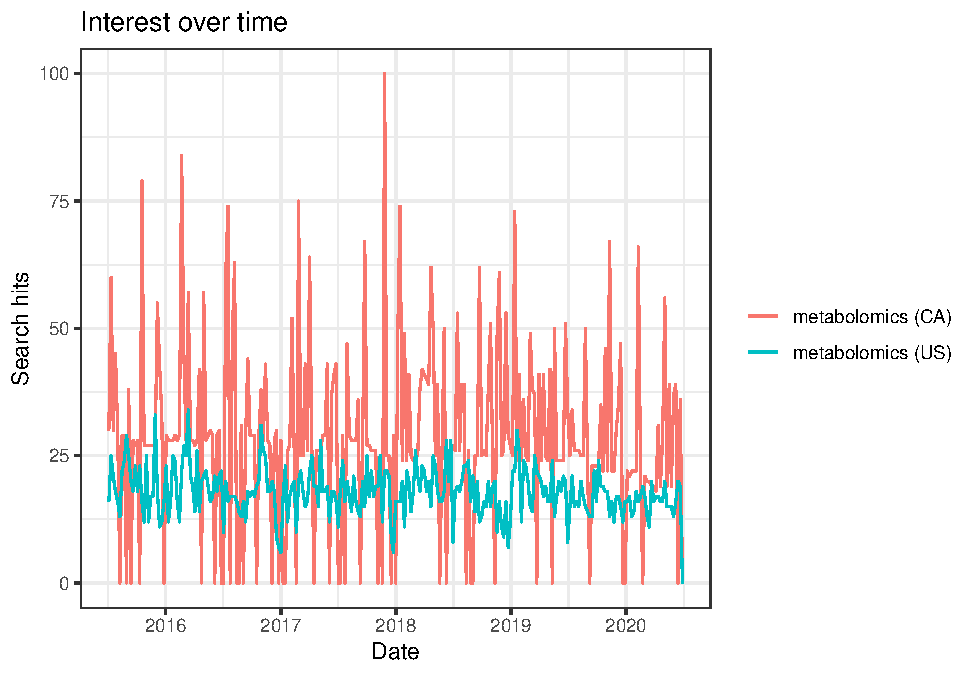
\includegraphics{Metabolomics_files/figure-latex/gtrends-1.pdf}

\begin{Shaded}
\begin{Highlighting}[]
\KeywordTok{library}\NormalTok{(rentrez)}
\NormalTok{papers_by_year <-}\StringTok{ }\ControlFlowTok{function}\NormalTok{(years, search_term)\{}
    \KeywordTok{return}\NormalTok{(}\KeywordTok{sapply}\NormalTok{(years, }\ControlFlowTok{function}\NormalTok{(y) }\KeywordTok{entrez_search}\NormalTok{(}\DataTypeTok{db=}\StringTok{"pubmed"}\NormalTok{,}\DataTypeTok{term=}\NormalTok{search_term, }\DataTypeTok{mindate=}\NormalTok{y, }\DataTypeTok{maxdate=}\NormalTok{y, }\DataTypeTok{retmax=}\DecValTok{0}\NormalTok{)}\OperatorTok{$}\NormalTok{count))}
\NormalTok{\}}
\NormalTok{years <-}\StringTok{ }\DecValTok{1987}\OperatorTok{:}\DecValTok{2018}
\NormalTok{total_papers <-}\StringTok{ }\KeywordTok{papers_by_year}\NormalTok{(years, }\StringTok{""}\NormalTok{)}
\NormalTok{omics <-}\StringTok{ }\KeywordTok{c}\NormalTok{(}\StringTok{"genomic"}\NormalTok{, }\StringTok{"epigenomic"}\NormalTok{,  }\StringTok{"metagenomic"}\NormalTok{, }\StringTok{"proteomic"}\NormalTok{, }\StringTok{"transcriptomic"}\NormalTok{,}\StringTok{"metabolomics"}\NormalTok{,}\StringTok{"exposome"}\NormalTok{, }\StringTok{"pharmacogenomic"}\NormalTok{, }\StringTok{"connectomic"}\NormalTok{)}
\NormalTok{trend_data <-}\StringTok{ }\KeywordTok{sapply}\NormalTok{(omics, }\ControlFlowTok{function}\NormalTok{(t) }\KeywordTok{papers_by_year}\NormalTok{(years, t))}
\NormalTok{trend_props <-}\StringTok{ }\NormalTok{trend_data}\OperatorTok{/}\NormalTok{total_papers}
\KeywordTok{library}\NormalTok{(reshape)}
\KeywordTok{library}\NormalTok{(ggplot2)}
\NormalTok{trend_df <-}\StringTok{ }\KeywordTok{melt}\NormalTok{(}\KeywordTok{data.frame}\NormalTok{(years, trend_data), }\DataTypeTok{id.vars=}\StringTok{"years"}\NormalTok{)}
\NormalTok{p <-}\StringTok{ }\KeywordTok{ggplot}\NormalTok{(trend_df, }\KeywordTok{aes}\NormalTok{(years, value, }\DataTypeTok{colour=}\NormalTok{variable))}
\NormalTok{p }\OperatorTok{+}\StringTok{ }\KeywordTok{geom_line}\NormalTok{(}\DataTypeTok{size=}\DecValTok{1}\NormalTok{) }\OperatorTok{+}\StringTok{ }\KeywordTok{scale_y_log10}\NormalTok{(}\StringTok{"number of papers"}\NormalTok{)}
\end{Highlighting}
\end{Shaded}

\begin{verbatim}
## Warning: Transformation introduced infinite values in
## continuous y-axis
\end{verbatim}

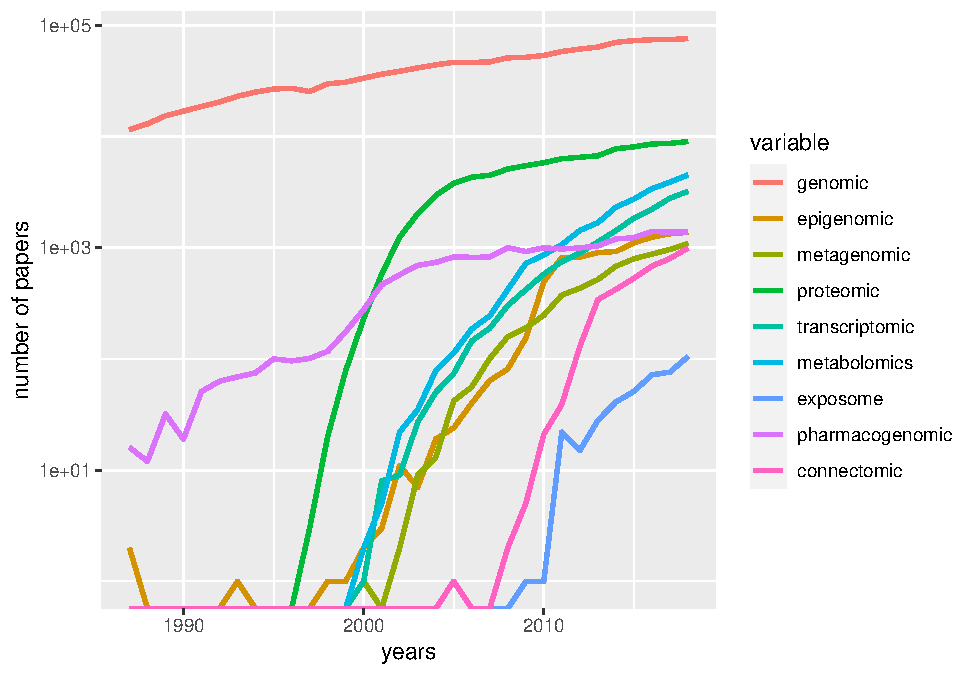
\includegraphics{Metabolomics_files/figure-latex/rentrez-1.pdf}

\hypertarget{workflow-1}{%
\section{Workflow}\label{workflow-1}}

\hypertarget{htmlwidget-26a18921f7f69567778e}{}

\hypertarget{experimental-designdoe}{%
\chapter{Experimental design(DoE)}\label{experimental-designdoe}}

Before you perform any metabolomics studies, a clean and meaningful experimental design is the best start. Depending on different research purposes, experiental design can be classified into homogeneity and heterogeneity study. Technique such as isotope labeled media will not be discussed in this chapter while this paper\citep{jang2018} could be a good start.

\hypertarget{homogeneity-study}{%
\section{Homogeneity study}\label{homogeneity-study}}

In homogeneity study, the research purpose is about method validation in most cases. Pooled sample made from multiple samples or technical replicates from same population will be used. Variances within the samples should be attibuted to factors other than the samples themselves. For example, one wants to test if sample injection order will affect the intensities of the unknown peaks. One pooled sample or technical replicates samples could be used here and the variances of the intensities should not be designed from heterogenety samples.

Another experimental design for homogeneity study will use biological replicates to find the common feasures from a group of samples. Biological replicates mean samples from same populatio with same biological process. For example, we wanted to know metabolites profiles of a certain species and we could collected lots of the individual samples from the same species. Then only the peaks/compounds appeared in all samples will be used to describe the metabolites profiles of this species. Technical replicates could also be used with biological replicates.

\hypertarget{heterogeneity-study}{%
\section{Heterogeneity study}\label{heterogeneity-study}}

In heterogeneity study, the research purpose is to find the differents among samples. To get the heterogeneity, you need at least a baseline to perform the comparision. Such baseline could be generated by random process or control samples or background knowledge. For example, outlier detection can be performed to find abnormal samples in unsupervised manners. Distribution or spatial analysis could be used to find geological relationship of known and unknown compounds. Temporal trend of metabolites profile could be found by time series or cohort studies. Clinical trial or random control trial is also an important class of heterogeneity studies. In this cases, you need at least two groups: treated group and control group. Also you could treat this group infomation as the one primary variable or primary variables to be explored for certain research purposes. In the following discussion about experimental design, we will use random control trail as model to discuss important issues.

\hypertarget{sample-size}{%
\section{Sample size}\label{sample-size}}

Supporsing we have control and treated groups, the numbers of samples in each group should be carefully calculated.For each metabolite, such comparision could be treated as one t-test. You need to perform a Power analysis to get the numbers. For example, we have two groups of samples with 10 samples in each group. Then we set the power at 0.9, which means one minus Type II error probability, the standard deviation at 1 and the significance level(Type 1 error probability) at 0.05. Then we get the meanful delta between the two groups should be higher than 1.53367 under this experiment design. Also we could set the delta to get the minimized numbers of the samples in each group. To get those data such as the standard deviation or delta for power analysis, you need to perform prelimitary or pilot experiments.

\begin{Shaded}
\begin{Highlighting}[]
\KeywordTok{power.t.test}\NormalTok{(}\DataTypeTok{n=}\DecValTok{10}\NormalTok{,}\DataTypeTok{sd=}\DecValTok{1}\NormalTok{,}\DataTypeTok{sig.level =} \FloatTok{0.05}\NormalTok{,}\DataTypeTok{power =} \FloatTok{0.9}\NormalTok{)}
\end{Highlighting}
\end{Shaded}

\begin{verbatim}
## 
##      Two-sample t test power calculation 
## 
##               n = 10
##           delta = 1.53367
##              sd = 1
##       sig.level = 0.05
##           power = 0.9
##     alternative = two.sided
## 
## NOTE: n is number in *each* group
\end{verbatim}

\begin{Shaded}
\begin{Highlighting}[]
\KeywordTok{power.t.test}\NormalTok{(}\DataTypeTok{delta =} \DecValTok{5}\NormalTok{,}\DataTypeTok{sd=}\DecValTok{1}\NormalTok{,}\DataTypeTok{sig.level =} \FloatTok{0.05}\NormalTok{,}\DataTypeTok{power =} \FloatTok{0.9}\NormalTok{)}
\end{Highlighting}
\end{Shaded}

\begin{verbatim}
## 
##      Two-sample t test power calculation 
## 
##               n = 2.328877
##           delta = 5
##              sd = 1
##       sig.level = 0.05
##           power = 0.9
##     alternative = two.sided
## 
## NOTE: n is number in *each* group
\end{verbatim}

However, since sometimes we could not perform preliminary experiment, we could directly compute the power based on false discovery rate control. If the power is lower than certain value, say 0.8, we just exclude this peak as significant features. In this review \citep{oberg2009}, author suggest to estimate an average \(\alpha\) according to this equation \citep{benjamini1995} and then use normal way to calculate the sample numbers:

\[
\alpha_{ave} \leq (1-\beta_{ave})\cdot q\frac{1}{1+(1-q)\cdot m_0/m_1}
\]

Other study \citep{blaise2016a} show a method based on simulation to estimate the sample size. They used BY correction to limit the influences from correlations. However, the nature of omics study make the power analysis hard to use one numbers for all metabolites and all the methods are trying to find a balance to represent more peaks with least samples(save money).

If there are other co-factors, a linear model or randomizing would be applied to eliminated their influences. You need to record the values of those co-factors for further data analysis. Common co-factors in metabolomics studies are age, gender, location, etc.

If you need data correction, some background or calibration samples are required. However, control samples could also be used for data correction in certain DoE.

Another important factors are instrumentals. High-resolution mass spectrum is always preferred. As shown in Lukas's study \citep{najdekr2016}:

\begin{quote}
the most effective mass resolving powers for profiling analyses of metabolite rich biofluids on the Orbitrap Elite were around 60000--120000 fwhm to retrieve the highest amount of information. The region between 400--800 m/z was influenced the most by resolution.
\end{quote}

However, elimination of peaks with high RSD\% within group were always omited by most study. Based on pre-experiment, you could get a description of RSD\% distribution and set cut-off to use stable peaks for further data analysis. To my knowledge, 50\% is suitable considering the batch effects.

\hypertarget{software}{%
\section{Software}\label{software}}

\begin{itemize}
\tightlist
\item
  \href{https://github.com/cran/MetSizeR}{MetSizeR} GUI Tool for Estimating Sample Sizes for metabolomics Experiments.
\end{itemize}

\hypertarget{pretreatment}{%
\chapter{Pretreatment}\label{pretreatment}}

Pretreatment will affect the results of metabolomics and cover the sample treatment from crude samples to injection vials. Sample pretreatment try to retain more interesting compounds while remove unrelated compounds. For metabolomics studies, we might not know `interesting' compounds in advance and the unrelated compounds are highly depended on research purpose. For example, Gel Permeation Chromatograph(GPC), Florisil, Alumina, Silica gel could be used to remove lipid while alcohols and strong acid/base could make protein denaturation to release more compounds. However, if we are interested in lipid or protein, such pretreatment methods should be changed. In general, sample quenching, extraction methods, derivatization, and storage should be optimized in pretreatment.

\hypertarget{quenching}{%
\section{Quenching}\label{quenching}}

Quenching solvent is always used to stop stop enzymatic activity.

In this review\citep{lu2017}, authors said:

\begin{quote}
A classical approach, which works well for many analytes, is boiling ethanol. Although the boiling solvent raises concerns about thermal degradation, it reliably denatures enzymes. In contrast, cold organic solvent may not fully denature enzymes or may do so too slowly such that some metabolic reactions continue, interconverting metabolites during the quenching process.
\end{quote}

This review\citep{kim2020} summarised the urease-dependent metabolome sample preparation and found:

\begin{quote}
activities of urease and endogenous urinary enzymes and metabolite contaminants from the urease preparations introduce artefacts into metabolite profiles, thus leading to misinterpretation.
\end{quote}

\hypertarget{extraction}{%
\section{Extraction}\label{extraction}}

According to this research\citep{bennett2009}:

\begin{quote}
The total metabolome concentration is approximately 300 mM, whereas the protein concentration is approximately 7 mM., which implies that most cellular metabolites are in free form.
\end{quote}

Dmitri et.al\citep{sitnikov2016} thought the most orthogonal methods to methanol-based precipitation were ion-exchange solid-phase extraction and liquid-liquid extraction using methyl-tertbutyl ether.

Tissue samples need to first be pulverized into fine powders.

Feces collected with 95\% ethanol or FOBT would be more reproducible and stable.

In this review\citep{lu2017}, authors said:

\begin{quote}
In our experience, for both cell and tissue specimens, 40:40:20 acetonitrile:methanol:water with 0.1 M formic acid (and subsequent neutralization with ammonium bicarbonate) is generally an effective solvent system for both quenching and extraction, including for ATP and other high-energy phosphorylated compounds. We typically use approximately 1 mL of solvent mix to extract 25 mg of biological specimen. \ldots Thus, although drying is acceptable for most metabolites, care must be taken with redox-active species.
\end{quote}

\citep{luo2017a} nano LC-MS could be used to analysis small numbers of cells.

For plant like soybeans\citep{mahmud2017}, ammonium acetate/methanol could be selected as extraction strategies compared with water/methanol and sodium phosphate/methanol.

\hypertarget{derivatization}{%
\section{Derivatization}\label{derivatization}}

Derivatization is always used in GC-based metabolomics study. This paper\citep{miyagawa2019} compared sequential derivatization methods and found different compounds would show different fluctuations during oximation or silylation process.

\hypertarget{storage}{%
\section{Storage}\label{storage}}

Samples should be stored after sample collection or sample pretreatment. -80°C or -20°C is always preferred to store samples. Dry ice should be used during sample pretreatment. However, comprehensive investigation of storage influnces found the metabolites profile will change after one day storage at -80°C. Rapid analysis of samples should be considered to capture more accurate information in the samples.

\hypertarget{instrumental-analysis}{%
\chapter{Instrumental analysis}\label{instrumental-analysis}}

To get more infomation in the samples, full scan is perferred on GC/LC-MS. Each scan would generat a mass spectrum to cover the setting mass range. If you narrow down your mass range and keep the same scan time, each mass would gain the collection time and you would get a higher sensitivity. However, if you expand your scan range, the sensitivity for each mass would decrease. You could also extend the collection time for each scan. However, it would affect the seperation process.

Full scan is performed synchronously with the seperation process. For a better seperation on chromotograph, each peak should have at least 10 point to get a nice peak shape. If you want to seperate two peaks with a retention time differences of 10s. Assuming the half peak width is 5s, you need to collect 10 mass spectrum within 10s. So the drwell time for each scan is 1s. If you use a high resolution column and the half peak width is 1s, you need to finish a scan within 0.2s. As we talked above, shorter drwell time would decrease the sensitivity. Thus there is a trade-off between seperation and sensitivity. If you use UPLC, the seperation could be finished within 20 min while you need to calculate if you mass spectrumetry could still show a good sensitivity.

\hypertarget{column-and-gradient-selection}{%
\section{Column and gradient selection}\label{column-and-gradient-selection}}

For GC, higher temperature could release compounds with higher boiling point. For LC, gradient and functional groups of stationary phase would be more important than temperature. Polarity of samples and column should match. More polar solvent could release polar compounds. Normal-phase column will not retain non-polar compounds while reversed-phase will elute polar column in the very beginning. To cover a wide polarity range or logP value compounds, normal phase column should match with non-polar to polar gradient to get a better seperation of polar compounds while reverse phase column should match with polar to non-polar gradient to elute compounds. If you use a inappropricate order of gradient, you compounds would not be seperated well. If you have no idea about column and gradient selection, literature's condiation might help.

\hypertarget{pooled-qc-samples}{%
\section{Pooled QC samples}\label{pooled-qc-samples}}

Pooled QC samples are unique and very important for metabolomics study. Every 10 or 20 samples, a pooled sample from all samples and blank sample in one study should be injected as quality control samples. Pooled QC samples contain the changes during the instrumental analysis and blank samples could tell where the variances come from. Meanwhile the cap of sequence should old the column with pooled QC samples. The injection sequence should be randomized. Those papers\citep{dunn2012, broadhurst2018} should be read for details.

\hypertarget{mass-resolution}{%
\section{Mass resolution}\label{mass-resolution}}

For metabolomics, high resolution mass spectrum should be used to make identification of compounds easier. The Mass Resolving Power is very important for annotation and high resolution mass spectrum should be calibrated in real time. The region between 400--800 m/z was influenced the most by resolution\citep{najdekr2016}. Orbitrap Fusion's performance was evaluated here\citep{barbiersainthilaire2018}.

\hypertarget{raw-data-pretreatment}{%
\chapter{Raw data pretreatment}\label{raw-data-pretreatment}}

Raw data from the instruments such as LC-MS or GC-MS were hard to be analyzed. To make it clear, the structure of those data could be summarised as:

\begin{itemize}
\item
  Indexed scan with time-stamp
\item
  Each scan contains a full scan mass spectra
\end{itemize}

Commen formats for open source mass spectrum data are mzxml, mzml or CDF. However, \textbf{masscomp} might shrink the data size\citep{yang2019b}.

\hypertarget{data-visualization}{%
\section{Data visualization}\label{data-visualization}}

You could use \href{https://salsa.debian.org/debichem-team/msxpertsuite}{msxpertsuite} for MS data visualization. It is biological mass spectrometry data visualization and mining with full JavaScript ability\citep{rusconi2019}.

\hypertarget{peak-extraction}{%
\section{Peak extraction}\label{peak-extraction}}

GC/LC-MS data are usually be shown as a matrix with column standing for retention times and row standing for masses after bin them into small cell.

\begin{figure}
\includegraphics[width=0.9\linewidth]{images/singledata} \caption{Demo of GC/LC-MS data}\label{fig:singledata}
\end{figure}

Conversation from the mass-retention time matrix into a vector with selected MS peaks at certain retention time is the basic idea of Peak extraction. You could EIC for each mass to charge ratio and use the change of trace slope to determine whether there is a peak or not. Then we could make integration for this peak and get peak area and retention time.

\begin{Shaded}
\begin{Highlighting}[]
\NormalTok{intensity <-}\StringTok{ }\KeywordTok{c}\NormalTok{(}\DecValTok{10}\NormalTok{,}\DecValTok{10}\NormalTok{,}\DecValTok{10}\NormalTok{,}\DecValTok{10}\NormalTok{,}\DecValTok{10}\NormalTok{,}\DecValTok{14}\NormalTok{,}\DecValTok{19}\NormalTok{,}\DecValTok{25}\NormalTok{,}\DecValTok{30}\NormalTok{,}\DecValTok{33}\NormalTok{,}\DecValTok{26}\NormalTok{,}\DecValTok{21}\NormalTok{,}\DecValTok{16}\NormalTok{,}\DecValTok{12}\NormalTok{,}\DecValTok{11}\NormalTok{,}\DecValTok{10}\NormalTok{,}\DecValTok{9}\NormalTok{,}\DecValTok{10}\NormalTok{,}\DecValTok{11}\NormalTok{,}\DecValTok{10}\NormalTok{)}
\NormalTok{time <-}\StringTok{ }\KeywordTok{c}\NormalTok{(}\DecValTok{1}\OperatorTok{:}\DecValTok{20}\NormalTok{)}
\KeywordTok{plot}\NormalTok{(intensity}\OperatorTok{~}\NormalTok{time, }\DataTypeTok{type =} \StringTok{'o'}\NormalTok{, }\DataTypeTok{main =} \StringTok{'EIC'}\NormalTok{)}
\end{Highlighting}
\end{Shaded}

\begin{figure}
\centering
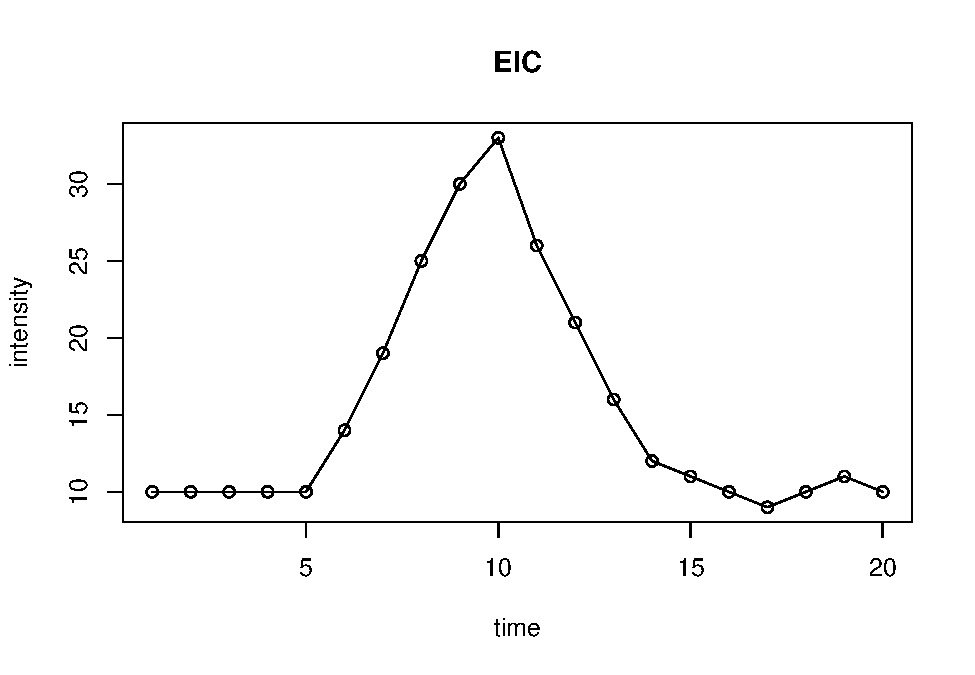
\includegraphics{Metabolomics_files/figure-latex/demoeic-1.pdf}
\caption{\label{fig:demoeic}Demo of EIC with peak}
\end{figure}

However, due to the accuracy of instrument, the detected mass to charge ratio would have some shift and EIC would fail if different scan get the intensity from different mass to charge ratio.

In the \texttt{matchedfilter} algorithm\citep{smith2006}, they solve this issue by bin the data in m/z dimension. The adjacent chromatographic slices could be combined to find a clean signal fitting fixed second-derivative Gaussian with full width at half-maximum
(fwhm) of 30s to find peaks with about 1.5-4 times the signal peak width. The the integration is performed on the fitted area.

\begin{figure}
\includegraphics[width=0.9\linewidth]{images/matchedfilter} \caption{Demo of matchedfilter}\label{fig:matchedfilter}
\end{figure}

The \texttt{Centwave} algorithm\citep{tautenhahn2008} based on detection of regions of interest(ROI) and the following Continuous Wavelet Transform (CWT) is preferred for high-resolution mass spectrum. ROI means a regine with stable mass for a certain time. When we find the ROIs, the peak shape is evaluated and ROI could be extended if needed. This algotithm use \texttt{prefilter} to accelerate the processing speed. \texttt{prefilter} with 3 and 100 means the ROI should contain 3 scan with intensity above 100. Centwave use a peak width range which should be checked on pool QC. Another important parameter is \texttt{ppm}. It is the maximum allowed deviation between scans when locating regions of interest (ROIs), which is different from vendor number and you need to extend them larger than the company claimed. For \texttt{profparam}, it's used for fill peaks or align peaks instead of peak picking. \texttt{snthr} is the cutoff of signal to noise ratio.

\hypertarget{retention-time-correction}{%
\section{Retention Time Correction}\label{retention-time-correction}}

For single file, we could get peaks. However, we should make the peaks align across samples for subsquece analysis and retention time corrections should be performed. The basic idea behind retention time correction is that use the high quality grouped peaks to make a new retention time. You might choose \texttt{obiwarp}(for dramatic shifts) or loess regression(fast) method to get the corrected retention time for all of the samples. Remember the original retention times might be changed and you might need cross-correct the data. After the correction, you could group the peaks again for a better cross-sample peaks list. However, if you directly use \texttt{obiwarp}, you don't have to group peaks before correction.

\citep{fu2017} show a matlab based shift correction methods.

\hypertarget{filling-missing-values}{%
\section{Filling missing values}\label{filling-missing-values}}

Too many zeros or NA in peaks list are problematic for statistics. Then we usually need to integreate the area exsiting a peak. \texttt{xcms\ 3} could use profile matrix to fill the blank. They also have function to impute the NA data by replace missing values with a proportion of the row minimum or random numbers based on the row minimum. It depends on the user to select imputation methods as well as control the minimum fraction of featuers appeared in single group.

\begin{figure}
\includegraphics[width=0.9\linewidth]{images/peakfiling} \caption{Peak filling of GC/LC-MS data}\label{fig:peakfilling}
\end{figure}

With many groups of samples, you will get another data matrix with column standing for peaks at cerntain retention time and row standing for samples after the Raw data pretreatment.

\begin{figure}
\includegraphics[width=0.9\linewidth]{images/multidata} \caption{Demo of many GC/LC-MS data}\label{fig:multidata}
\end{figure}

\hypertarget{spectral-deconvolution}{%
\section{Spectral deconvolution}\label{spectral-deconvolution}}

Without fracmental infomation about certain compound, the peak extraction would suffer influnces from other compounds. At the same retention time, co-elute compounds might share similar mass. Hard electron ionization methods such as electron impact ionization (EI), APPI suffer this issue. So it would be hard to distighuish the co-elute peaks' origin and deconvolution method\citep{du2013} could be used to seperate different groups according to the similar chromatogragh beheviors. Another computational tool \textbf{eRah} could be a better solution for the whole process\citep{domingo-almenara2016}. Also the \textbf{ADAD-GC3.0} could also be helpful for such issue\citep{ni2016}.

\hypertarget{dynamic-range}{%
\section{Dynamic Range}\label{dynamic-range}}

Another issue is the Dynamic Range. For metabolomics, peaks could be below the detection limit or over the detection limit. Such Dynamic range issues might raise the loss of information.

\hypertarget{non-detects}{%
\subsection{Non-detects}\label{non-detects}}

Some of the data were limited by the detect of limitation. Thus we need some methods to impute the data if we don't want to lose information by deleting the NA or 0.

Two major imputation way could be used. The first way is use model-free method such as half the minimum of the values across the data, 0, 1, mean/median across the data( \texttt{enviGCMS} package could do this via \texttt{getimputation} function). The second way is use model-based method such as linear model, random forest, KNN, PCA. Try \texttt{simputation} package for various imputation methods. As mentioned before, you could also use \texttt{imputeRowMin} or \texttt{imputeRowMinRand} within \texttt{xcms} package to perform imputation.

Tobit regression is preferred for censored data. Also you might choose maximum likelihood estimation(Estimation of mean and standard deviation by MLE. Creating 10 complete samples. Pool the results from 10 individual analyses).

\begin{Shaded}
\begin{Highlighting}[]
\NormalTok{x <-}\StringTok{ }\KeywordTok{rnorm}\NormalTok{(}\DecValTok{1000}\NormalTok{,}\DecValTok{1}\NormalTok{)}
\NormalTok{x[x}\OperatorTok{<}\DecValTok{0}\NormalTok{] <-}\StringTok{ }\DecValTok{0}
\NormalTok{y <-}\StringTok{ }\NormalTok{x}\OperatorTok{*}\DecValTok{10}\OperatorTok{+}\DecValTok{1}
\KeywordTok{library}\NormalTok{(AER)}
\NormalTok{tfit <-}\StringTok{ }\KeywordTok{tobit}\NormalTok{(y }\OperatorTok{~}\StringTok{ }\NormalTok{x, }\DataTypeTok{left =} \DecValTok{0}\NormalTok{)}
\KeywordTok{summary}\NormalTok{(tfit)}
\end{Highlighting}
\end{Shaded}

\begin{verbatim}
## 
## Call:
## tobit(formula = y ~ x, left = 0)
## 
## Observations:
##          Total  Left-censored     Uncensored Right-censored 
##           1000              0           1000              0 
## 
## Coefficients:
##             Estimate Std. Error z value Pr(>|z|)    
## (Intercept)   1.0000     0.4310    2.32   0.0203 *  
## x            10.0000     0.3162   31.62   <2e-16 ***
## Log(scale)    2.1501     0.0000     Inf   <2e-16 ***
## ---
## Signif. codes:  
## 0 '***' 0.001 '**' 0.01 '*' 0.05 '.' 0.1 ' ' 1
## 
## Scale: 8.586 
## 
## Gaussian distribution
## Number of Newton-Raphson Iterations: 1 
## Log-likelihood: -3069 on 3 Df
## Wald-statistic:  1000 on 1 Df, p-value: < 2.22e-16
\end{verbatim}

According to Ronald Hites's simulation\citep{hites2019}, measurements below the LOD (even missing measurements) with the LOD/2 or with the \(LOD/\sqrt2\) causes little bias and ``Any time you have a \% non-detected \textgreater20\%, for whatever reason, it is unlikely that the data set can give useful results.''

\hypertarget{over-detection-limit}{%
\subsection{Over Detection Limit}\label{over-detection-limit}}

\textbf{CorrectOverloadedPeaks} could be used to correct the Peaks Exceeding the Detection Limit issue\citep{lisec2016}.

\hypertarget{rsdfold-change-filter}{%
\section{RSD/fold change Filter}\label{rsdfold-change-filter}}

Some peaks need to be rule out due to high RSD\% and small fold changes compared with blank samples.

\hypertarget{power-analysis-filter}{%
\section{Power Analysis Filter}\label{power-analysis-filter}}

As shown in {[}Exprimental design(DoE){]}, the power analysis in metabolomics is ad-hoc since you don't know too much before you perform the experiment. However, we could perform power analysis after the experiment done. That is, we just rule out the peaks with a lower power in exsit Exprimental design.

\hypertarget{software-1}{%
\section{Software}\label{software-1}}

\hypertarget{peak-picking}{%
\subsection{Peak picking}\label{peak-picking}}

\begin{itemize}
\item
  \href{http://proteowizard.sourceforge.net/}{ProteoWizard Toolkit} provides a set of open-source, cross-platform software libraries and tools \citep{chambers2012}. Msconvert is one tool in this toolkit.
\item
  \href{https://github.com/sneumann/xcms}{xcms} LC/MS and GC/MS Data Analysis\citep{smith2006}
\item
  \href{https://sourceforge.net/projects/aplcms/}{apLCMS} Generate peaks list \citep{yu2009}
\item
  \href{http://pubs.acs.org/doi/10.1021/ac403384n}{x13cms} global tracking of isotopic labels in untargeted metabolomics \citep{huang2014}
\item
  \href{https://github.com/wkew/FTMSVisualization}{FTMSVisualization} is a suite of tools for visualizing complex mixture FT-MS data\citep{kew2017}
\item
  \href{http://mzmine.github.io/}{MZmine} is an open-source software for mass-spectrometry data processing, with the main focus on LC-MS data\citep{pluskal2010}
\item
  \href{http://prime.psc.riken.jp/Metabolomics_Software/}{MS-DAIL} is a universal program for untargeted metabolomics- and lipidomics supporting any type of chromatography/mass spectrometry methods (GC/MS, GC-MS/MS, LC/MS, and LC-MS/MS etc.) \citep{tsugawa2015}
\item
  \href{http://www.openms.de/}{OpenMS} is an open-source software C++ library for LC/MS data management and analyses\citep{rost2016}
\item
  \href{https://sourceforge.net/projects/mzmatch/}{MZmatch} is a Java collection of small commandline tools specific for metabolomics MS data analysis \citep{scheltema2011, creek2012}
\item
  \href{http://ms.iis.sinica.edu.tw/comics/Software_iMet-Q.html}{iMet-Q} is an automated tool with friendly user interfaces for quantifying metabolites in full-scan liquid chromatography-mass spectrometry (LC-MS) data.\citep{chang2016}
\item
  \href{http://genomics-pubs.princeton.edu/mzroll/index.php}{MAVEN} is an open source cross platform metabolomics data analyser.\citep{melamud2010}
\end{itemize}

\hypertarget{for-msms}{%
\subsection{For MS/MS}\label{for-msms}}

\begin{itemize}
\item
  \href{http://prime.psc.riken.jp/Metabolomics_Software/}{MS-DAIL} for data independent MS/MS deconvolution of comprehensive metabolome analysis.\citep{tsugawa2015}
\item
  \href{https://pubs.acs.org/doi/10.1021/ac400751j}{decoMS2} An Untargeted Metabolomic Workflow to Improve Structural Characterization of Metabolites\citep{nikolskiy2013}
\item
  \href{https://pubs.acs.org/doi/10.1021/acs.analchem.6b04358}{msPurity} Automated Evaluation of Precursor Ion Purity for Mass Spectrometry-Based Fragmentation in Metabolomics\citep{lawson2017}
\item
  \href{https://pubs.acs.org/doi/suppl/10.1021/acs.est.8b00259/suppl_file/es8b00259_si_001.pdf}{ULSA} Deconvolution algorithm and a universal library search algorithm (ULSA) for the analysis of complex spectra generated via data-independent acquisition based on Matlab \citep{samanipour2018}
\end{itemize}

\hypertarget{improved-peak-picking}{%
\subsection{Improved Peak picking}\label{improved-peak-picking}}

\begin{itemize}
\item
  \href{https://github.com/rietho/IPO}{IPO} A Tool for automated Optimization of XCMS Parameters\citep{libiseller2015}.
\item
  \href{https://github.com/nathaniel-mahieu/warpgroup}{Warpgroup} is used for chromatogram subregion detection, consensus integration bound determination and accurate missing value integration\citep{mahieu2016}
\item
  \href{https://bmcbioinformatics.biomedcentral.com/articles/10.1186/1471-2105-14-15}{xMSanalyzer} improved Peak picking for xcms and apLCMS\citep{uppal2013}
\item
  \href{https://bitbucket.org/fiehnlab/ms-flo/src/657d85ec7bdd?at=master}{ms-flo} A Tool To Minimize False Positive Peak Reports in Untargeted Liquid Chromatography--Mass Spectroscopy (LC-MS) Data Processing\citep{defelice2017}
\end{itemize}

\hypertarget{tips}{%
\section{Tips}\label{tips}}

\begin{itemize}
\tightlist
\item
  Convert XCMSnExp object into xcmsSet object
\end{itemize}

\begin{Shaded}
\begin{Highlighting}[]
\NormalTok{xcmsSetdemo <-}\StringTok{ }\KeywordTok{as}\NormalTok{(XCMSnExpdemo,}\StringTok{'xcmsSet'}\NormalTok{)}
\end{Highlighting}
\end{Shaded}

\begin{itemize}
\tightlist
\item
  Split xcmsSet with multiple groups object into a list with single group object
\end{itemize}

\begin{Shaded}
\begin{Highlighting}[]
\NormalTok{list <-}\StringTok{ }\KeywordTok{split}\NormalTok{(xcmsSetdemo,xcmsSetdemo}\OperatorTok{@}\NormalTok{phenoData}\OperatorTok{$}\NormalTok{sample_group)}
\CommentTok{# re-group the peaks with parallel computation}
\NormalTok{list2 <-}\StringTok{ }\NormalTok{BiocParallel}\OperatorTok{::}\KeywordTok{bplapply}\NormalTok{(list,group)}
\end{Highlighting}
\end{Shaded}

\begin{itemize}
\tightlist
\item
  Combine single group xcmsSet objects into one xcmsSet
\end{itemize}

\begin{Shaded}
\begin{Highlighting}[]
\NormalTok{xcmsSetdemoagain <-}\StringTok{ }\KeywordTok{Reduce}\NormalTok{(}\StringTok{'c'}\NormalTok{,list2)}
\CommentTok{# for more higher order function in R, check here: http://www.johnmyleswhite.com/notebook/2010/09/23/higher-order-functions-in-r/}
\end{Highlighting}
\end{Shaded}

\begin{itemize}
\tightlist
\item
  Use \textbf{warpgroup} to get peaks with better quality
\end{itemize}

\begin{Shaded}
\begin{Highlighting}[]
\KeywordTok{library}\NormalTok{(doParallel)}
\NormalTok{cl =}\StringTok{ }\KeywordTok{makeCluster}\NormalTok{(}\KeywordTok{detectCores}\NormalTok{() }\OperatorTok{-}\StringTok{ }\DecValTok{1}\NormalTok{)}
\KeywordTok{registerDoParallel}\NormalTok{(cl)}

\NormalTok{xseteiclist =}\StringTok{ }\KeywordTok{lapply}\NormalTok{(xcmsSetdemo}\OperatorTok{@}\NormalTok{filepaths, xcmsRaw, }\DataTypeTok{profstep=}\DecValTok{0}\NormalTok{)}
\NormalTok{xwarpgroup =}\StringTok{ }\KeywordTok{group.warpgroup}\NormalTok{(xcmsSetdemo, xseteiclist, }\DataTypeTok{rt.max.drift =} \DecValTok{20}\NormalTok{, }\DataTypeTok{ppm.max.drift =} \DecValTok{3}\NormalTok{, }\DataTypeTok{rt.aligned.lim =} \DecValTok{5}\NormalTok{)}
\end{Highlighting}
\end{Shaded}

\hypertarget{peaks-normalization}{%
\chapter{Peaks normalization}\label{peaks-normalization}}

\hypertarget{batch-effects-classification}{%
\section{Batch effects classification}\label{batch-effects-classification}}

Variances among the samples across all the extracted peaks might be affected by factors other than the experiment design. There are three types of those batch effects: Monotone, Block and Mixed.

\begin{itemize}
\tightlist
\item
  Monotone would increase/decrease with the injection order or batchs.
\end{itemize}

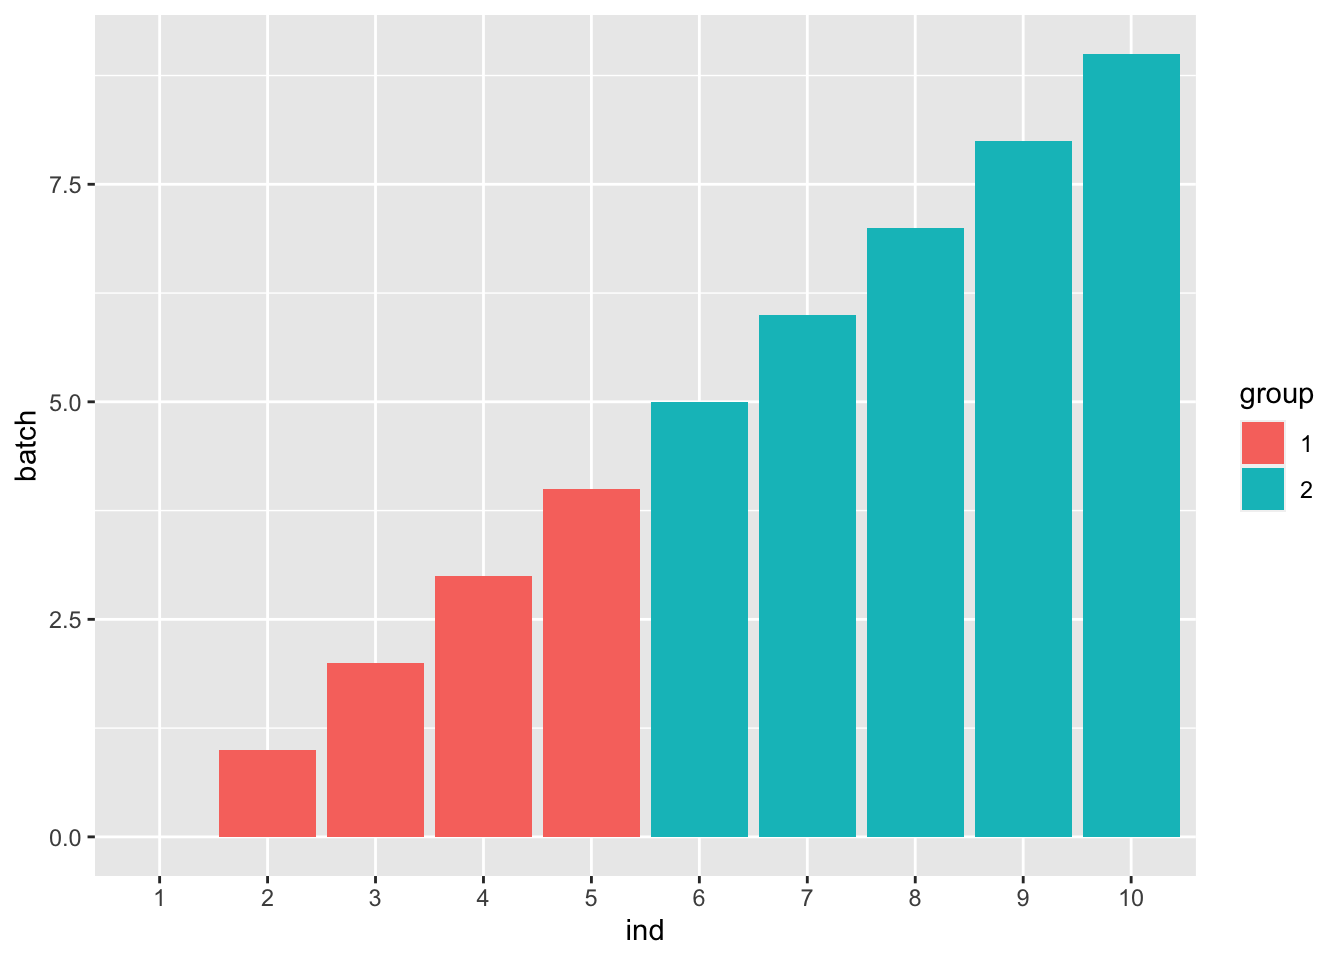
\includegraphics[width=0.618\linewidth]{Metabolomics_files/figure-latex/unnamed-chunk-8-1}

\begin{itemize}
\tightlist
\item
  Block would be system shift among different batchs.
\end{itemize}

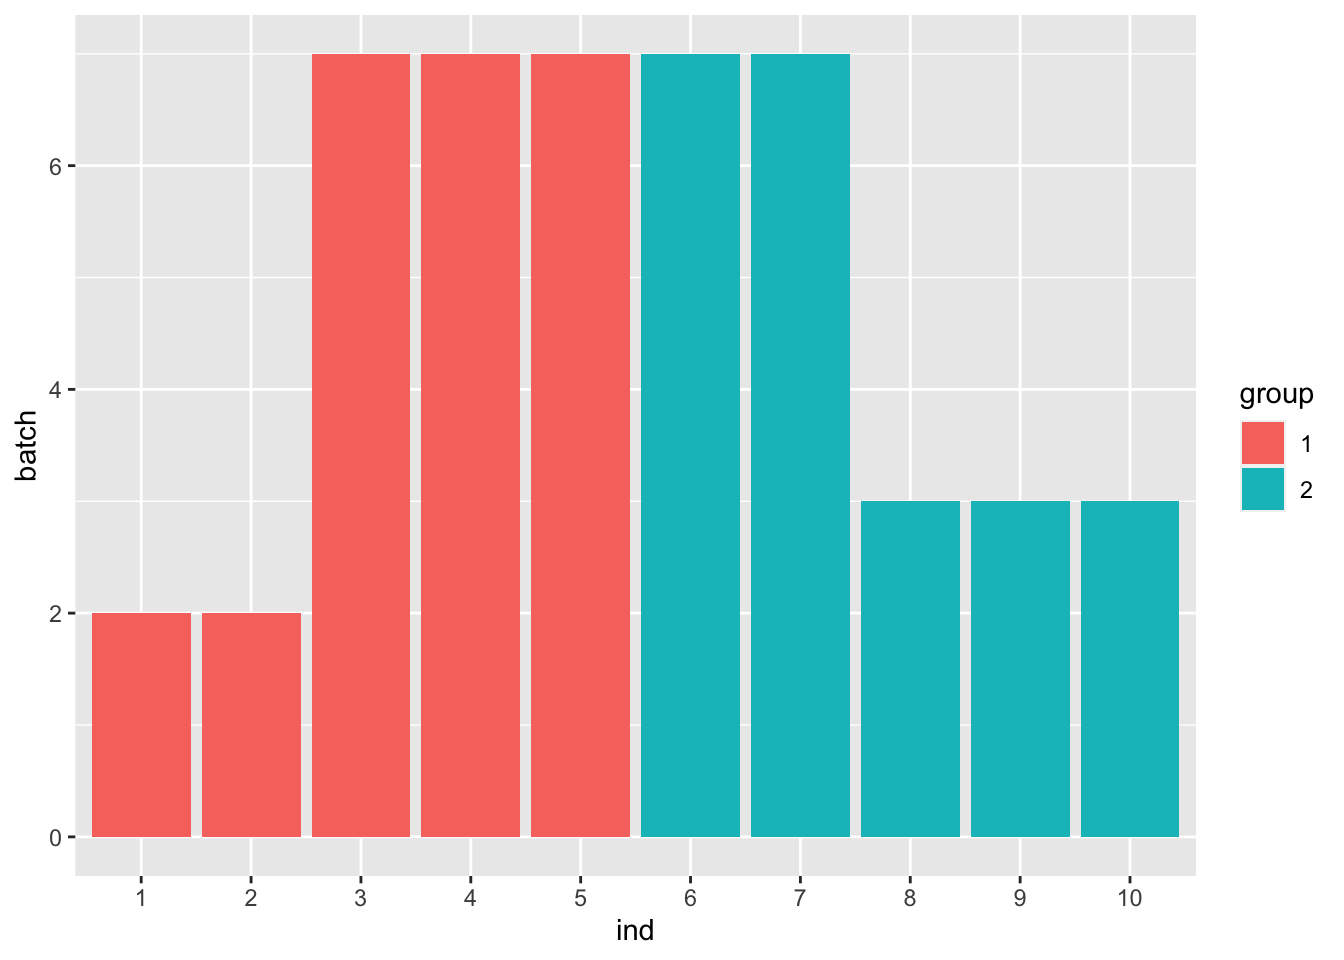
\includegraphics[width=0.618\linewidth]{Metabolomics_files/figure-latex/unnamed-chunk-9-1}

\begin{itemize}
\tightlist
\item
  Mixed would be the combination of monotone and block batch effects.
\end{itemize}

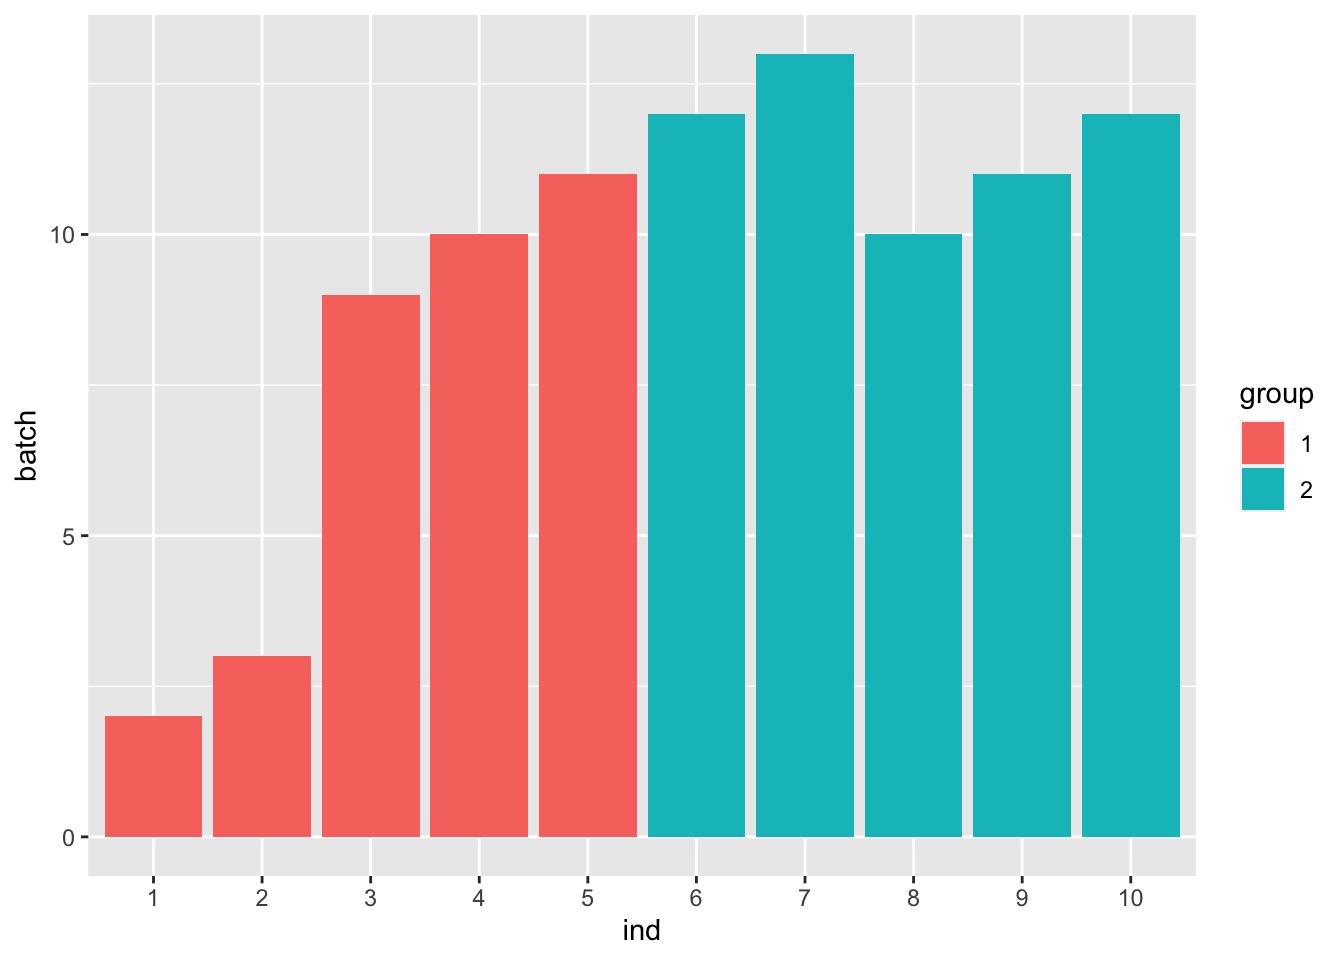
\includegraphics[width=0.618\linewidth]{Metabolomics_files/figure-latex/unnamed-chunk-10-1}

Meanwhile, different compounds would suffer different type of batch effects. In this case, the normalization or batch correction should be done peak by peak.

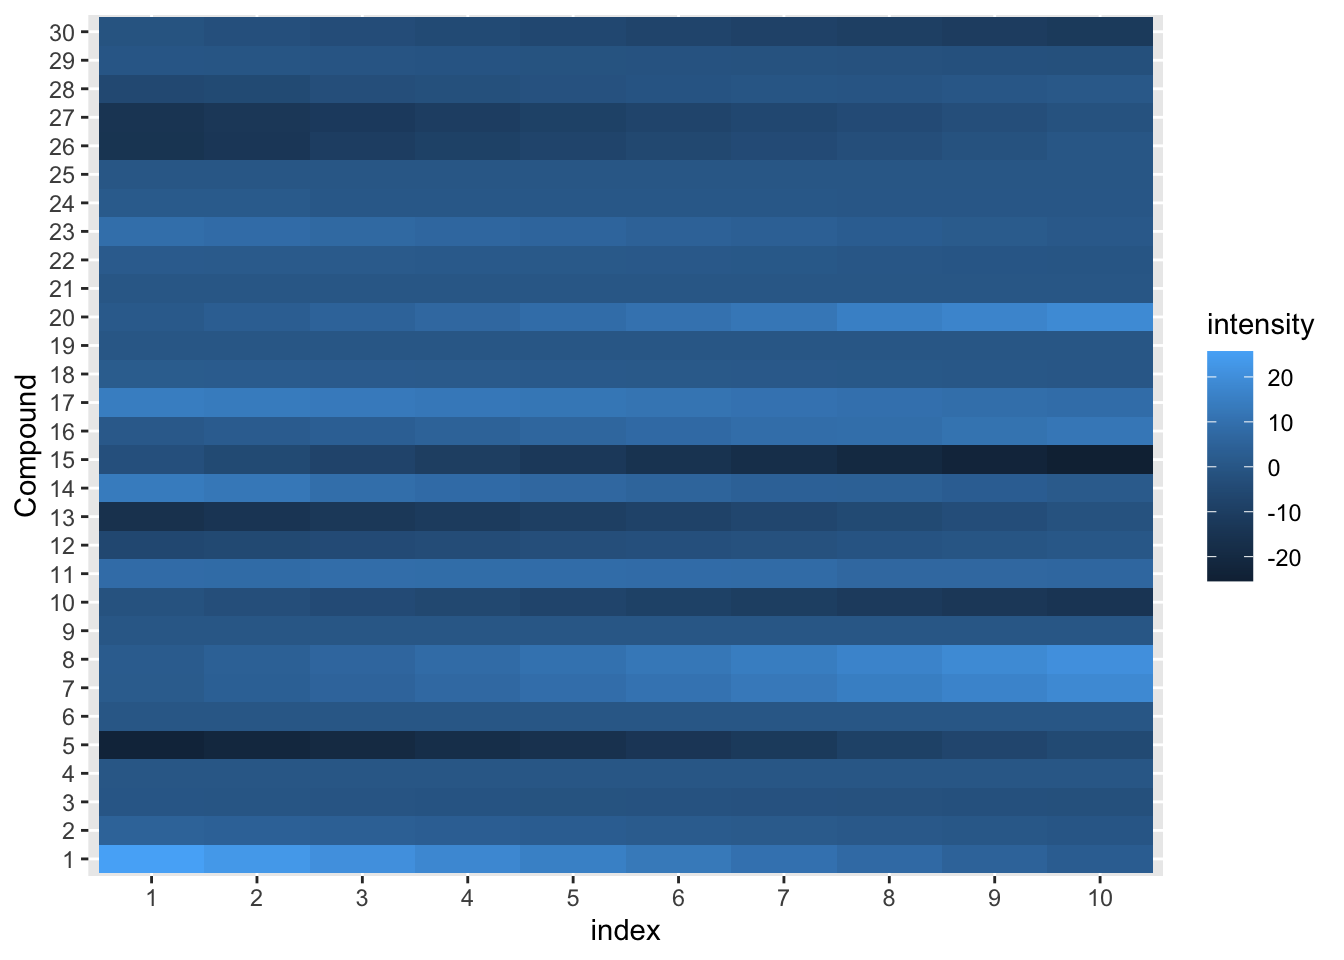
\includegraphics[width=0.7\linewidth]{Metabolomics_files/figure-latex/bem-1}

\hypertarget{batch-effects-visulization}{%
\section{Batch effects visulization}\label{batch-effects-visulization}}

Any correction might introduce bias. We need to make sure there are patterns which different from our experimental design. Pooled QC samples should be clustered on PCA score plot.

\hypertarget{source-of-batch-effects}{%
\section{Source of batch effects}\label{source-of-batch-effects}}

\begin{itemize}
\item
  Different Operators \& Dates \& Sequences
\item
  Different Instrumental Condition such as different instrumental parameters, poor quality control, sample contamination during the analysis, Column (Pooled QC) and sample matrix effects (ions suppression or/and enhancement)
\item
  Unknown Unknowns
\end{itemize}

\hypertarget{avoid-batch-effects-by-doe}{%
\section{Avoid batch effects by DoE}\label{avoid-batch-effects-by-doe}}

You could avoid batch effects from experimental design. Cap the sequence with Pooled QC and Randomized samples sequence. Some internal standards/Instrumental QC might Help to find the source of batch effects while it's not practical for every compounds in non-targeted analysis.

Batch effects might not change the conclusion when the effect size is relatively small. Here is a simulation:

\begin{Shaded}
\begin{Highlighting}[]
\KeywordTok{set.seed}\NormalTok{(}\DecValTok{30}\NormalTok{)}
\CommentTok{# real peaks}
\NormalTok{group <-}\StringTok{ }\KeywordTok{factor}\NormalTok{(}\KeywordTok{c}\NormalTok{(}\KeywordTok{rep}\NormalTok{(}\DecValTok{1}\NormalTok{,}\DecValTok{5}\NormalTok{),}\KeywordTok{rep}\NormalTok{(}\DecValTok{2}\NormalTok{,}\DecValTok{5}\NormalTok{)))}
\NormalTok{con <-}\StringTok{ }\KeywordTok{c}\NormalTok{(}\KeywordTok{rnorm}\NormalTok{(}\DecValTok{5}\NormalTok{,}\DecValTok{5}\NormalTok{),}\KeywordTok{rnorm}\NormalTok{(}\DecValTok{5}\NormalTok{,}\DecValTok{8}\NormalTok{))}
\NormalTok{re <-}\StringTok{ }\KeywordTok{t.test}\NormalTok{(con}\OperatorTok{~}\NormalTok{group)}
\CommentTok{# real peaks}
\NormalTok{group <-}\StringTok{ }\KeywordTok{factor}\NormalTok{(}\KeywordTok{c}\NormalTok{(}\KeywordTok{rep}\NormalTok{(}\DecValTok{1}\NormalTok{,}\DecValTok{5}\NormalTok{),}\KeywordTok{rep}\NormalTok{(}\DecValTok{2}\NormalTok{,}\DecValTok{5}\NormalTok{)))}
\NormalTok{con <-}\StringTok{ }\KeywordTok{c}\NormalTok{(}\KeywordTok{rnorm}\NormalTok{(}\DecValTok{5}\NormalTok{,}\DecValTok{5}\NormalTok{),}\KeywordTok{rnorm}\NormalTok{(}\DecValTok{5}\NormalTok{,}\DecValTok{8}\NormalTok{))}
\NormalTok{batch <-}\StringTok{ }\KeywordTok{seq}\NormalTok{(}\DecValTok{0}\NormalTok{,}\DecValTok{5}\NormalTok{,}\DataTypeTok{length.out =} \DecValTok{10}\NormalTok{)}
\NormalTok{ins <-}\StringTok{ }\NormalTok{batch}\OperatorTok{+}\NormalTok{con}
\NormalTok{re <-}\StringTok{ }\KeywordTok{t.test}\NormalTok{(ins}\OperatorTok{~}\NormalTok{group)}

\NormalTok{index <-}\StringTok{ }\KeywordTok{sample}\NormalTok{(}\DecValTok{10}\NormalTok{)}
\NormalTok{ins <-}\StringTok{ }\NormalTok{batch}\OperatorTok{+}\NormalTok{con[index]}
\NormalTok{re <-}\StringTok{ }\KeywordTok{t.test}\NormalTok{(ins}\OperatorTok{~}\NormalTok{group[index])}
\end{Highlighting}
\end{Shaded}

Randomization could not guarantee the results. Here is a simulation.

\begin{Shaded}
\begin{Highlighting}[]
\CommentTok{# real peaks}
\NormalTok{group <-}\StringTok{ }\KeywordTok{factor}\NormalTok{(}\KeywordTok{c}\NormalTok{(}\KeywordTok{rep}\NormalTok{(}\DecValTok{1}\NormalTok{,}\DecValTok{5}\NormalTok{),}\KeywordTok{rep}\NormalTok{(}\DecValTok{2}\NormalTok{,}\DecValTok{5}\NormalTok{)))}
\NormalTok{con <-}\StringTok{ }\KeywordTok{c}\NormalTok{(}\KeywordTok{rnorm}\NormalTok{(}\DecValTok{5}\NormalTok{,}\DecValTok{5}\NormalTok{),}\KeywordTok{rnorm}\NormalTok{(}\DecValTok{5}\NormalTok{,}\DecValTok{8}\NormalTok{))}
\NormalTok{batch <-}\StringTok{ }\KeywordTok{seq}\NormalTok{(}\DecValTok{5}\NormalTok{,}\DecValTok{0}\NormalTok{,}\DataTypeTok{length.out =} \DecValTok{10}\NormalTok{)}
\NormalTok{ins <-}\StringTok{ }\NormalTok{batch}\OperatorTok{+}\NormalTok{con}
\NormalTok{re <-}\StringTok{ }\KeywordTok{t.test}\NormalTok{(ins}\OperatorTok{~}\NormalTok{group)}
\end{Highlighting}
\end{Shaded}

\hypertarget{post-hoc-data-normalization}{%
\section{post hoc data normalization}\label{post-hoc-data-normalization}}

To make the samples comparable, normailization across the samples are always needed when the experiment part is done. Batch effect should have patterns, otherwise just noise. Correction is possible by data analysis/randomized experimental design. There are more than 20 methods to make normalization. We could devided those methods into two category: unsupervised and supervised.

Unsupervised methods only consider the normalization peaks intensity distribution across the samples. For example, quantile calibration try to make the intensity distribution among the samples similar. Such methods are preferred to explore the inner structures of the samples. Internal standards or pool QC samples also belong to this category. However, it's hard to take a few peaks standing for all peaks extracted.

Supervised methods will use the group information or batch information in experimental design to normalize the data. A linear model is always used to model the unwanted variances and remove them for further analysis.

Since the real batch effects are always unknown, it's hard to make validation for different normalization methods. Wu et.al preferred to make comparision between new methods and conventional methods\citep{wu2016}. Li et.al developed NOREVA to make comparision among 25 correction method\citep{li2017a}. Another idea is use spiked-in samples to validate the methods\citep{franceschi2012}, which might be good for targeted analysis instead of non-targeted analysis.

Relative log abundance (RLA) plots\citep{delivera2012} and heatmap often used to show the variances among the samples.

\citep{thonusin2017} some methods for batch correction in excel

\hypertarget{unsupervised-methods}{%
\subsection{Unsupervised methods}\label{unsupervised-methods}}

\hypertarget{distribution-of-intensity}{%
\subsubsection{Distribution of intensity}\label{distribution-of-intensity}}

Intensity collects from LC/GC-MS always showed a right-skewed distribution. Log transformation is often necessary for further statistical analysis.

\hypertarget{centering}{%
\subsubsection{Centering}\label{centering}}

For peak p of sample s in batch b, the corrected abundance I is:

\[\hat I_{p,s,b} = I_{p,s,b} - mean(I_{p,b}) + median(I_{p,qc})\]

If no quality control samples used, the corrected abundance I would be:

\[\hat I_{p,s,b} = I_{p,s,b} - mean(I_{p,b})\]

\hypertarget{scaling}{%
\subsubsection{Scaling}\label{scaling}}

For peak p of sample s in certain batch b, the corrected abundance I is:

\[\hat I_{p,s,b} = \frac{I_{p,s,b} - mean(I_{p,b})}{std_{p,b}} * std_{p,qc,b} + mean(I_{p,qc,b})\]
If no quality control samples used, the corrected abundance I would be:

\[\hat I_{p,s,b} = \frac{I_{p,s,b} - mean(I_{p,b})}{std_{p,b}}\]

\hypertarget{pareto-scaling}{%
\subsubsection{Pareto Scaling}\label{pareto-scaling}}

For peak p of sample s in certain batch b, the corrected abundance I is:

\[\hat I_{p,s,b} = \frac{I_{p,s,b} - mean(I_{p,b})}{Sqrt(std_{p,b})} * Sqrt(std_{p,qc,b}) + mean(I_{p,qc,b})\]

If no quality control samples used, the corrected abundance I would be:

\[\hat I_{p,s,b} = \frac{I_{p,s,b} - mean(I_{p,b})}{Sqrt(std_{p,b})}\]

\hypertarget{range-scaling}{%
\subsubsection{Range Scaling}\label{range-scaling}}

For peak p of sample s in certain batch b, the corrected abundance I is:

\[\hat I_{p,s,b} = \frac{I_{p,s,b} - mean(I_{p,b})}{max(I_{p,b}) - min(I_{p,b})} * (max(I_{p,qc,b}) - min(I_{p,qc,b})) + mean(I_{p,qc,b})\]

If no quality control samples used, the corrected abundance I would be:

\[\hat I_{p,s,b} = \frac{I_{p,s,b} - mean(I_{p,b})}{max(I_{p,b}) - min(I_{p,b})} \]

\hypertarget{level-scaling}{%
\subsubsection{Level scaling}\label{level-scaling}}

For peak p of sample s in certain batch b, the corrected abundance I is:

\[\hat I_{p,s,b} = \frac{I_{p,s,b} - mean(I_{p,b})}{mean(I_{p,b})} * mean(I_{p,qc,b}) + mean(I_{p,qc,b})\]

If no quality control samples used, the corrected abundance I would be:

\[\hat I_{p,s,b} = \frac{I_{p,s,b} - mean(I_{p,b})}{mean(I_{p,b})} \]

\hypertarget{quantile}{%
\subsubsection{Quantile}\label{quantile}}

The idea of quantile calibration is that alignment of the intensities in certain samples according to quantiles in each sample.

Here is the demo:

\begin{Shaded}
\begin{Highlighting}[]
\KeywordTok{set.seed}\NormalTok{(}\DecValTok{42}\NormalTok{)}
\NormalTok{a <-}\StringTok{ }\KeywordTok{rnorm}\NormalTok{(}\DecValTok{1000}\NormalTok{)}
\CommentTok{# b sufferred batch effect with a bias of 10}
\NormalTok{b <-}\StringTok{ }\KeywordTok{rnorm}\NormalTok{(}\DecValTok{1000}\NormalTok{,}\DecValTok{10}\NormalTok{)}
\KeywordTok{hist}\NormalTok{(a,}\DataTypeTok{xlim=}\KeywordTok{c}\NormalTok{(}\OperatorTok{-}\DecValTok{5}\NormalTok{,}\DecValTok{15}\NormalTok{),}\DataTypeTok{breaks =} \DecValTok{50}\NormalTok{)}
\KeywordTok{hist}\NormalTok{(b,}\DataTypeTok{col =} \StringTok{'black'}\NormalTok{, }\DataTypeTok{breaks =} \DecValTok{50}\NormalTok{, }\DataTypeTok{add=}\NormalTok{T)}
\CommentTok{# quantile normalized}
\NormalTok{cor <-}\StringTok{ }\NormalTok{(a[}\KeywordTok{order}\NormalTok{(a)]}\OperatorTok{+}\NormalTok{b[}\KeywordTok{order}\NormalTok{(b)])}\OperatorTok{/}\DecValTok{2}
\CommentTok{# reorder}
\NormalTok{cor <-}\StringTok{ }\NormalTok{cor[}\KeywordTok{order}\NormalTok{(}\KeywordTok{order}\NormalTok{(a))]}
\KeywordTok{hist}\NormalTok{(cor,}\DataTypeTok{col =} \StringTok{'red'}\NormalTok{, }\DataTypeTok{breaks =} \DecValTok{50}\NormalTok{, }\DataTypeTok{add=}\NormalTok{T)}
\end{Highlighting}
\end{Shaded}

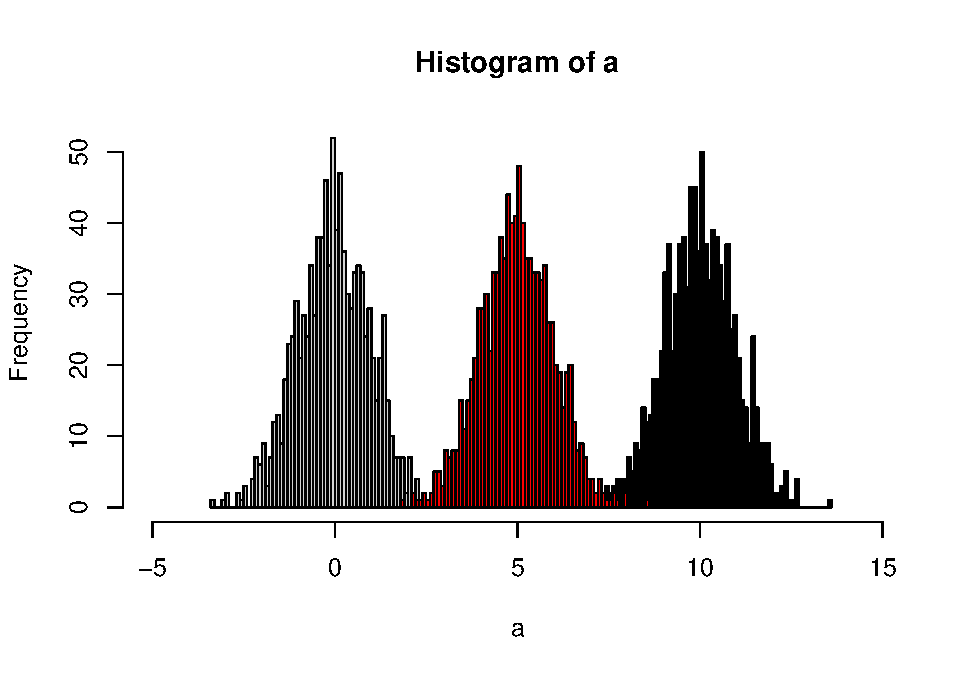
\includegraphics{Metabolomics_files/figure-latex/quantile-1.pdf}

\hypertarget{ratio-based-calibraton}{%
\subsubsection{Ratio based calibraton}\label{ratio-based-calibraton}}

This method calibrates samples by the ratio between qc samples in all samples and in certain batch.For peak p of sample s in certain batch b, the corrected abundance I is:

\[\hat I_{p,s,b} = \frac{I_{p,s,b} * median(I_{p,qc})}{mean_{p,qc,b}}\]

\begin{Shaded}
\begin{Highlighting}[]
\KeywordTok{set.seed}\NormalTok{(}\DecValTok{42}\NormalTok{)}
\CommentTok{# raw data}
\NormalTok{I =}\StringTok{ }\KeywordTok{c}\NormalTok{(}\KeywordTok{rnorm}\NormalTok{(}\DecValTok{10}\NormalTok{,}\DataTypeTok{mean =} \DecValTok{0}\NormalTok{, }\DataTypeTok{sd =} \FloatTok{0.3}\NormalTok{),}\KeywordTok{rnorm}\NormalTok{(}\DecValTok{10}\NormalTok{,}\DataTypeTok{mean =} \DecValTok{1}\NormalTok{, }\DataTypeTok{sd =} \FloatTok{0.5}\NormalTok{))}
\CommentTok{# batch}
\NormalTok{B =}\StringTok{ }\KeywordTok{c}\NormalTok{(}\KeywordTok{rep}\NormalTok{(}\DecValTok{0}\NormalTok{,}\DecValTok{10}\NormalTok{),}\KeywordTok{rep}\NormalTok{(}\DecValTok{1}\NormalTok{,}\DecValTok{10}\NormalTok{))}
\CommentTok{# qc}
\NormalTok{Iqc =}\StringTok{ }\KeywordTok{c}\NormalTok{(}\KeywordTok{rnorm}\NormalTok{(}\DecValTok{1}\NormalTok{,}\DataTypeTok{mean =} \DecValTok{0}\NormalTok{, }\DataTypeTok{sd =} \FloatTok{0.3}\NormalTok{),}\KeywordTok{rnorm}\NormalTok{(}\DecValTok{1}\NormalTok{,}\DataTypeTok{mean =} \DecValTok{1}\NormalTok{, }\DataTypeTok{sd =} \FloatTok{0.5}\NormalTok{))}
\CommentTok{# corrected data}
\NormalTok{Icor =}\StringTok{ }\NormalTok{I }\OperatorTok{*}\StringTok{ }\KeywordTok{median}\NormalTok{(}\KeywordTok{c}\NormalTok{(}\KeywordTok{rep}\NormalTok{(Iqc[}\DecValTok{1}\NormalTok{],}\DecValTok{10}\NormalTok{),}\KeywordTok{rep}\NormalTok{(Iqc[}\DecValTok{2}\NormalTok{],}\DecValTok{10}\NormalTok{)))}\OperatorTok{/}\KeywordTok{mean}\NormalTok{(}\KeywordTok{c}\NormalTok{(}\KeywordTok{rep}\NormalTok{(Iqc[}\DecValTok{1}\NormalTok{],}\DecValTok{10}\NormalTok{),}\KeywordTok{rep}\NormalTok{(Iqc[}\DecValTok{2}\NormalTok{],}\DecValTok{10}\NormalTok{)))}
\CommentTok{# plot the result}
\KeywordTok{plot}\NormalTok{(I)}
\end{Highlighting}
\end{Shaded}

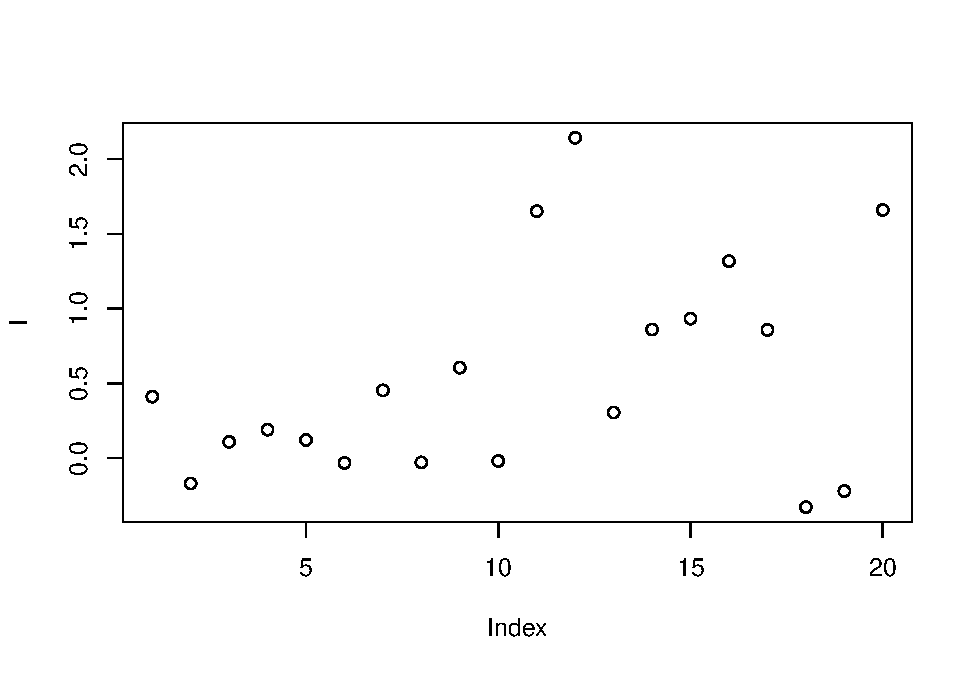
\includegraphics{Metabolomics_files/figure-latex/ratio-1.pdf}

\begin{Shaded}
\begin{Highlighting}[]
\KeywordTok{plot}\NormalTok{(Icor)}
\end{Highlighting}
\end{Shaded}

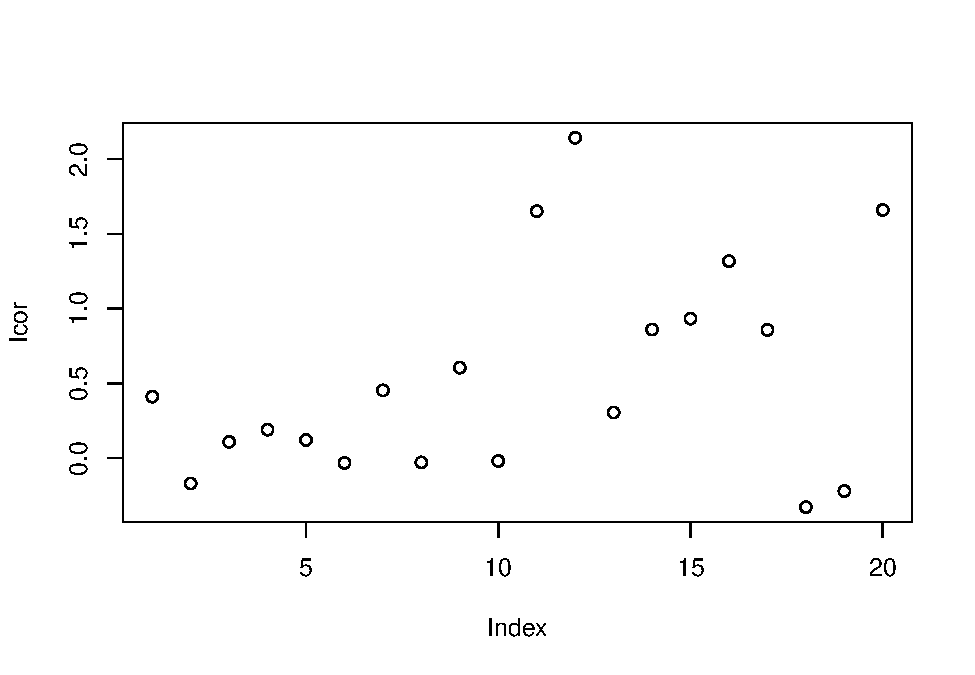
\includegraphics{Metabolomics_files/figure-latex/ratio-2.pdf}

\hypertarget{linear-normalizer}{%
\subsubsection{Linear Normalizer}\label{linear-normalizer}}

This method initially scales each sample so that the sum of all
peak abundances equals one. In this study, by multiplying the median sum of all peak abundances across all samples,we got the corrected data.

\begin{Shaded}
\begin{Highlighting}[]
\KeywordTok{set.seed}\NormalTok{(}\DecValTok{42}\NormalTok{)}
\CommentTok{# raw data}
\NormalTok{peaksa <-}\StringTok{ }\KeywordTok{c}\NormalTok{(}\KeywordTok{rnorm}\NormalTok{(}\DecValTok{10}\NormalTok{,}\DataTypeTok{mean =} \DecValTok{10}\NormalTok{, }\DataTypeTok{sd =} \FloatTok{0.3}\NormalTok{),}\KeywordTok{rnorm}\NormalTok{(}\DecValTok{10}\NormalTok{,}\DataTypeTok{mean =} \DecValTok{20}\NormalTok{, }\DataTypeTok{sd =} \FloatTok{0.5}\NormalTok{))}
\NormalTok{peaksb <-}\StringTok{ }\KeywordTok{c}\NormalTok{(}\KeywordTok{rnorm}\NormalTok{(}\DecValTok{10}\NormalTok{,}\DataTypeTok{mean =} \DecValTok{10}\NormalTok{, }\DataTypeTok{sd =} \FloatTok{0.3}\NormalTok{),}\KeywordTok{rnorm}\NormalTok{(}\DecValTok{10}\NormalTok{,}\DataTypeTok{mean =} \DecValTok{20}\NormalTok{, }\DataTypeTok{sd =} \FloatTok{0.5}\NormalTok{))}

\NormalTok{df <-}\StringTok{ }\KeywordTok{rbind}\NormalTok{(peaksa,peaksb)}
\NormalTok{dfcor <-}\StringTok{ }\NormalTok{df}\OperatorTok{/}\KeywordTok{apply}\NormalTok{(df,}\DecValTok{2}\NormalTok{,sum)}\OperatorTok{*}\StringTok{ }\KeywordTok{sum}\NormalTok{(}\KeywordTok{apply}\NormalTok{(df,}\DecValTok{2}\NormalTok{,median))}

\KeywordTok{image}\NormalTok{(df)}
\end{Highlighting}
\end{Shaded}

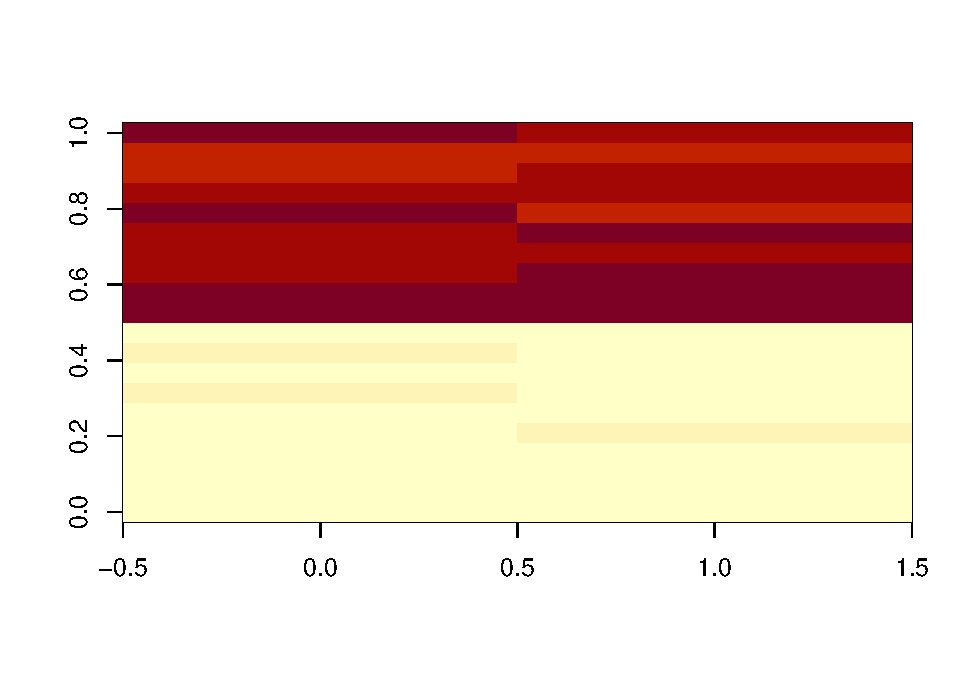
\includegraphics{Metabolomics_files/figure-latex/Linear-1.pdf}

\begin{Shaded}
\begin{Highlighting}[]
\KeywordTok{image}\NormalTok{(dfcor)}
\end{Highlighting}
\end{Shaded}

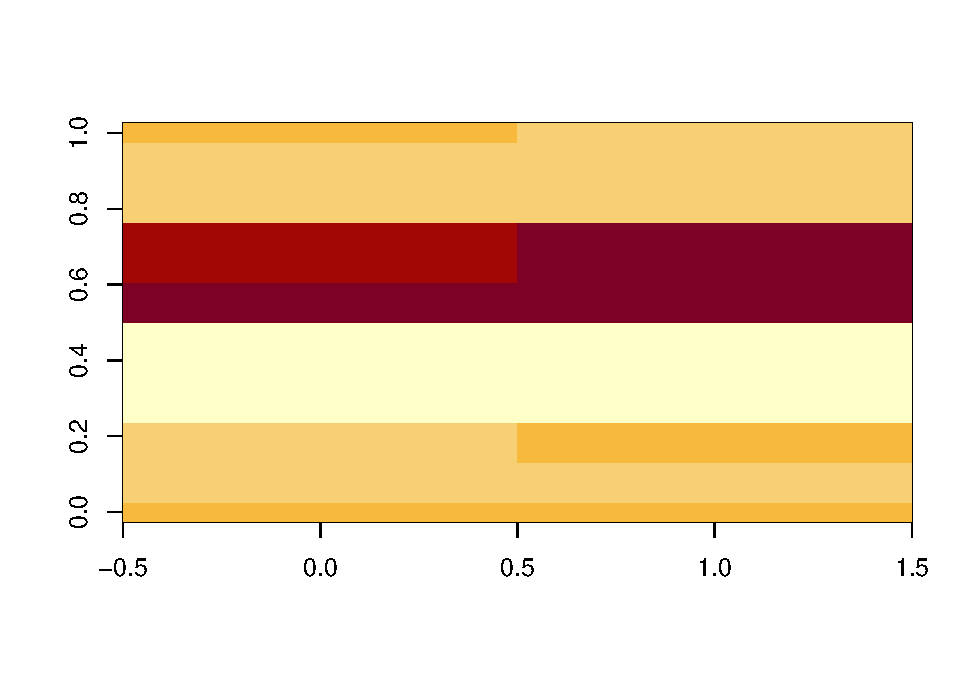
\includegraphics{Metabolomics_files/figure-latex/Linear-2.pdf}

\hypertarget{internal-standards}{%
\subsubsection{Internal standards}\label{internal-standards}}

\[\hat I_{p,s} = \frac{I_{p,s} * median(I_{IS})}{I_{IS,s}}\]

Some methods also use pooled calibration samples and multiple internal standard strategy to correct the data\citep{van_der_kloet2009}. Also some methods only use QC samples to handle the data\citep{kuligowski2015}.

\hypertarget{supervised-methods}{%
\subsection{Supervised methods}\label{supervised-methods}}

\hypertarget{regression-calibration}{%
\subsubsection{Regression calibration}\label{regression-calibration}}

Considering the batch effect of injection order, regress the data by a linear model to get the calibration.

\hypertarget{batch-normalizer}{%
\subsubsection{Batch Normalizer}\label{batch-normalizer}}

Use the total abundance scale and then fit with the regression line\citep{wang2013}.

\hypertarget{surrogate-variable-analysissva}{%
\subsubsection{Surrogate Variable Analysis(SVA)}\label{surrogate-variable-analysissva}}

We have a data matrix(M*N) with M stands for indentity peaks from one sample and N stand for individual samples. For one sample, \(X = (x_{i1},...,x_{in})^T\) stands for the normalized intensities of peaks. We use \(Y = (y_i,...,y_m)^T\) stands for the group infomation of our data. Then we could build such modles:

\[x_{ij} = \mu_i + f_i(y_i) + e_{ij}\]

\(\mu_i\) stands for the baseline of the peak intensities in a normal state. Then we have:

\[f_i(y_i) = E(x_{ij}|y_j) - \mu_i\]

stands for the biological variations caused by the our group, for example, whether treated by pollutions or not.

However, considering the batch effects, the real model could be:

\[x_{ij} = \mu_i + f_i(y_i) + \sum_{l = 1}^L \gamma_{li}p_{lj} + e_{ij}^*\]
\(\gamma_{li}\) stands for the peak-specific coefficient for potentical factor \(l\). \(p_{lj}\) stands for the potential factors across the samples. Actually, the error item \(e_{ij}\) in real sample could always be decomposed as \(e_{ij} = \sum_{l = 1}^L \gamma_{li}p_{lj} + e_{ij}^*\) with \(e_{ij}^*\) standing for the real random error in certain sample for certain peak.

We could not get the potential factors directly. Since we don't care the details of the unknown factors, we could estimate orthogonal vectors \(h_k\) standing for such potential factors. Thus we have:

\[
x_{ij} = \mu_i + f_i(y_i) + \sum_{l = 1}^L \gamma_{li}p_{lj} + e_{ij}^*\\ 
= \mu_i + f_i(y_i) + \sum_{k = 1}^K \lambda_{ki}h_{kj} + e_{ij}
\]

Here is the details of the algorithm:

\begin{quote}
The algorithm is decomposed into two parts: detection of unmodeled factors and construction of surrogate variables
\end{quote}

\hypertarget{detection-of-unmodeled-factors}{%
\paragraph{Detection of unmodeled factors}\label{detection-of-unmodeled-factors}}

\begin{itemize}
\item
  Estimate \(\hat\mu_i\) and \(f_i\) by fitting the model \(x_{ij} = \mu_i + f_i(y_i) + e_{ij}\) and get the residual \(r_{ij} = x_{ij}-\hat\mu_i - \hat f_i(y_i)\). Then we have the residual matrix R.
\item
  Perform the singular value decompositon(SVD) of the residual matrix \(R = UDV^T\)
\item
  Let \(d_l\) be the \(l\)th eigenvalue of the diagonal matrix D for \(l = 1,...,n\). Set \(df\) as the freedom of the model \(\hat\mu_i + \hat f_i(y_i)\). We could build a statistic \(T_k\) as:
\end{itemize}

\[T_k = \frac{d_k^2}{\sum_{l=1}^{n-df}d_l^2}\]

to show the variance explained by the \(k\)th eigenvalue.

\begin{itemize}
\item
  Permute each row of R to remove the structure in the matrix and get \(R^*\).
\item
  Fit the model \(r_{ij}^* = \mu_i^* + f_i^*(y_i) + e^*_{ij}\) and get \(r_{ij}^0 = r^*_{ij}-\hat\mu^*_i - \hat f^*_i(y_i)\) as a null matrix \(R_0\)
\item
  Perform the singular value decompositon(SVD) of the residual matrix \(R_0 = U_0D_0V_0^T\)
\item
  Compute the null statistic:
\end{itemize}

\[
T_k^0 = \frac{d_{0k}^2}{\sum_{l=1}^{n-df}d_{0l}^2}
\]

\begin{itemize}
\item
  Repeat permuting the row B times to get the null statistics \(T_k^{0b}\)
\item
  Get the p-value for eigengene:
\end{itemize}

\[p_k = \frac{\#{T_k^{0b}\geq T_k;b=1,...,B }}{B}\]

\begin{itemize}
\tightlist
\item
  For a significance level \(\alpha\), treat k as a significant signature of residual R if \(p_k\leq\alpha\)
\end{itemize}

\hypertarget{construction-of-surrogate-variables}{%
\paragraph{Construction of surrogate variables}\label{construction-of-surrogate-variables}}

\begin{itemize}
\item
  Estimate \(\hat\mu_i\) and \(f_i\) by fitting the model \(x_{ij} = \mu_i + f_i(y_i) + e_{ij}\) and get the residual \(r_{ij} = x_{ij}-\hat\mu_i - \hat f_i(y_i)\). Then we have the residual matrix R.
\item
  Perform the singular value decompositon(SVD) of the residual matrix \(R = UDV^T\). Let \(e_k = (e_{k1},...,e_{kn})^T\) be the \(k\)th column of V
\item
  Set \(\hat K\) as the significant eigenvalues found by the first step.
\item
  Regress each \(e_k\) on \(x_i\), get the p-value for the association.
\item
  Set \(\pi_0\) as the proportion of the peak intensitity \(x_i\) not associate with \(e_k\) and find the numbers \(\hat m =[1-\hat \pi_0 \times m]\) and the indices of the peaks associated with the eigenvalues
\item
  Form the matrix \(\hat m_1 \times N\), this matrix\(X_r\) stand for the potiential variables. As was done for R, get the eigengents of \(X_r\) and denote these by \(e_j^r\)
\item
  Let \(j^* = argmax_{1\leq j \leq n}cor(e_k,e_j^r)\) and set \(\hat h_k=e_j^r\). Set the estimate of the surrogate variable to be the eigenvalue of the reduced matrix most correlated with the corresponding residual eigenvalue. Since the reduced matrix is enriched for peaks associated with this residual eigenvalue, this is a principled choice for the estimated surrogate variable that allows for correlation with the primary variable.
\item
  Employ the \(\mu_i + f_i(y_i) + \sum_{k = 1}^K \gamma_{ki}\hat h_{kj} + e_{ij}\) as te estimate of the ideal model \(\mu_i + f_i(y_i) + \sum_{k = 1}^K \gamma_{ki}h_{kj} + e_{ij}\)
\end{itemize}

This method could found the potentical unwanted variables for the data. SVA were introduced by Jeff Leek\citep{leek2012, leek2007, leek2008} and EigenMS package implement SVA with modifications including analysis of data with missing values that are typical in LC-MS experiments\citep{karpievitch2014a}.

\hypertarget{ruv-remove-unwanted-variation}{%
\subsubsection{RUV (Remove Unwanted Variation)}\label{ruv-remove-unwanted-variation}}

This method's performance is similar to SVA. Instead find surrogate variable from the whole dataset. RUA use control or pool QC to find the unwanted variances and remove them to find the peaks related to experimental design. However, we could also empirically estimate the control peaks by linear mixed model. RUA-random\citep{livera2015} furthor use linear mixed model to estimate the variances of random error. This method could be used with suitable control, which is commen in metabolomics DoE.

\hypertarget{rrmix}{%
\subsubsection{RRmix}\label{rrmix}}

RRmix also use a latent factor models correct the data\citep{jr2017}. This method could be treated as linear mixed model version SVA. No control samples are required and the unwanted variances could be removed by factor analysis. This method might be the best choise to remove the unwanted variables with commen experiment design.

\hypertarget{method-to-validate-the-normalization}{%
\section{Method to validate the normalization}\label{method-to-validate-the-normalization}}

\hypertarget{software-2}{%
\section{Software}\label{software-2}}

\begin{itemize}
\item
  \href{https://github.com/rwehrens/BatchCorrMetabolomics}{BatchCorrMetabolomics} is for improved batch correction in untargeted MS-based metabolomics
\item
  \href{https://github.com/cran/MetNorm}{MetNorm} show Statistical Methods for Normalizing Metabolomics Data.
\item
  \href{https://github.com/mani2012/BatchQC}{BatchQC} could be used to make batch effect simulation.
\item
  \href{http://idrb.zju.edu.cn/noreva/}{Noreva} could make online batch correction.
\end{itemize}

\hypertarget{annotation}{%
\chapter{Annotation}\label{annotation}}

When you get the peaks table or features table, annotation of the peaks would help you. Check this review\citep{domingo-almenara2018} for a detailed notes on annotation. They proposed five levels regarding currently computational annotation strategies.

\begin{itemize}
\item
  Level 1: Peak Grouping: MS Psedospectra extraction based on peak shape similarity and peak abundance correlation
\item
  Level 2: Peak Annotation: Adducts, Neutral losses, isotopes, and other mass relationships based on mass distances
\item
  Level 3: Biochemical knowledge based on putative identification, potential biochemical reaction and related statistical analysis
\item
  Level 4: Use and intergration of tandem MS data based on data dependant/independent acquistion mode or \textbf{in silico} predction
\item
  Level 5: Retention time prediction based on library-available retention index or quantitative structure-retnetion relationships (QSRR) models.
\end{itemize}

Most of the softwares are at level 1 or 2. If we only have compounds structure, we could guess ions under different ionization method. If we have mass spectrum, we could match the mass spectral by a similarity analysis to the database. In metabolomics, we only have mass spectrum or mass-to-charge ratios. Single mass-to-charge ratio is not enough for identification. That's the one bottleneck for annotation. So prediction is always performed on MS/MS data.

\hypertarget{issues-in-annotation}{%
\section{Issues in annotation}\label{issues-in-annotation}}

The major issue in annotation is the redundancy peaks from same metabolite. Unlike genomcis, peaks or featuers from peak selection are not independant with each other. Adducts, in-source fragments and isotopes would lead to missannotation. A commen solution is that use known adducts, neutral losses, molecular multimers or multipley charged ions to compare mass distances.

Another issue is about the MS/MS database. Only 10\% of known metabolites in databases have experimental spectral data. Thus \textbf{in silico} prediction are required. Some works try to fill the gap between experimental data, theoretical values(from chemical database like chemspider) and prediction together. Here is a nice review about MS/MS prediction\citep{hufsky2014}.

\hypertarget{peak-misidentification}{%
\section{Peak misidentification}\label{peak-misidentification}}

\begin{itemize}
\tightlist
\item
  Isomer
\end{itemize}

Use seperation methods such as chromatography, ion mobility MS, MS/MS. Reversed-phase ion-pairing chromatography and HILIC is useful.Chemical derivatization is another options.

\begin{itemize}
\tightlist
\item
  Interfering compounds
\end{itemize}

20ppm is the least resolution and accuracy for HRMS.

\begin{itemize}
\tightlist
\item
  In-source degradation products
\end{itemize}

\hypertarget{annotation-v.s.-identification}{%
\section{Annotation v.s. identification}\label{annotation-v.s.-identification}}

According to the defination from the Chemical Analysis Working Group of the Metabolomics Standards Intitvative\citep{sumner2007, viant2017}. Four levels of confidence could be assigned to identification:

\begin{itemize}
\tightlist
\item
  Level 1 `identified metabolites'
\item
  Level 2 `Putatively annotated compounds'
\item
  Level 3 `Putatively characterised compound classes'
\item
  Level 4 `Unknown'
\end{itemize}

In practice, data analysis based annotation could reach level 2. For level 1, we need at extra methods such as MS/MS, retention time, accurate mass, 2D NMR spectra, and so on to confirm the compounds. However, standards are always required for solid proof.

\hypertarget{cheminformatics}{%
\section{Cheminformatics}\label{cheminformatics}}

\begin{itemize}
\tightlist
\item
  \href{https://www.rdkit.org/}{RDKit} Open-Source Cheminformatics Software
\item
  \href{https://sourceforge.net/projects/cdk/}{cdk} The Chemistry Development Kit (CDK) is a scientific, LGPL-ed library for bio- and cheminformatics and computational chemistry written in Java.
\item
  \href{http://openbabel.org/wiki/Main_Page}{Open Babel} Open Babel is a chemical toolbox designed to speak the many languages of chemical data.
\end{itemize}

\hypertarget{ms-database-for-annotation}{%
\section{MS Database for annotation}\label{ms-database-for-annotation}}

\hypertarget{msms}{%
\subsection{MS/MS}\label{msms}}

\begin{itemize}
\item
  \href{http://mona.fiehnlab.ucdavis.edu/}{MoNA} Platform to collect all other open source database
\item
  \href{http://www.massbank.jp/?lang=en}{MassBank}
\item
  \href{https://gnps.ucsd.edu/ProteoSAFe/static/gnps-splash.jsp}{GNPS} use inner correlationship in the data and make network analysis at peaks' level instand of annotated compounds to annotate the data\citep{wang2016b}.
\item
  \href{http://spectra.psc.riken.jp/}{ReSpect}: phytochemicals
\item
  \href{https://metlin.scripps.edu/}{Metlin} is another useful online application for annotation\citep{guijas2018}.
\item
  \href{http://fiehnlab.ucdavis.edu/projects/LipidBlast}{LipidBlast}: in silico prediction
\item
  \href{https://www.mzcloud.org/}{MZcloud}
\item
  \href{https://www.nist.gov/srd/nist-standard-reference-database-1a-v17}{NIST}: Not free
\end{itemize}

\hypertarget{ms}{%
\subsection{MS}\label{ms}}

\begin{itemize}
\item
  \href{http://fiehnlab.ucdavis.edu/projects/binbase-setup}{Fiehn Lab}
\item
  \href{https://www.nist.gov/srd/nist-standard-reference-database-1a-v17}{NIST}: No free
\item
  \href{https://sdbs.db.aist.go.jp/sdbs/cgi-bin/cre_index.cgi?lang=eng}{Spectral Database for Organic Compounds, SDBS}
\item
  \href{http://minedatabase.mcs.anl.gov/\#/faq}{MINE} is an open access database of computationally predicted enzyme promiscuity products for untargeted metabolomics
\item
  \href{https://www.sciencedirect.com/science/article/abs/pii/S0039914019311786?via\%3Dihub}{Database} of free solution mobilities for 276 metabolites for capillary zone electrophoresis / mass spectrometry. \citep{petrov2020}
\end{itemize}

\hypertarget{compounds-database}{%
\section{Compounds Database}\label{compounds-database}}

\begin{itemize}
\item
  \href{https://pubchem.ncbi.nlm.nih.gov/}{PubChem} is an open chemistry database at the National Institutes of Health (NIH).
\item
  \href{http://www.chemspider.com/}{Chemspider} is a free chemical structure database providing fast text and structure search access to over 67 million structures from hundreds of data sources.
\item
  \href{https://www.ebi.ac.uk/chebi/}{ChEBI} is a freely available dictionary of molecular entities focused on `small' chemical compounds.
\item
  \href{http://www.metabolomicsworkbench.org/databases/refmet/index.php}{RefMet} A Reference list of Metabolite names.
\item
  \href{https://www.cas.org/support/documentation/chemical-substances/cas-registry-100-millionth-fun-facts}{CAS} Largest substance database
\end{itemize}

\hypertarget{software-3}{%
\section{Software}\label{software-3}}

\hypertarget{adducts-list}{%
\subsection{Adducts list}\label{adducts-list}}

You could find adducts list \href{https://github.com/stanstrup/commonMZ}{here} from commonMZ project.

\hypertarget{molgen}{%
\subsection{Molgen}\label{molgen}}

\href{http://molgen.de}{molgen} generating all structures (connectivity isomers, constitutions) that correspond to a given molecular formula, with optional further restrictions, e.g.~presence or absence of particular substructures.

\hypertarget{isotope}{%
\subsection{Isotope}\label{isotope}}

\href{https://www.envipat.eawag.ch/index.php}{Isotope} pattern prediction

\hypertarget{mffinder}{%
\subsection{mfFinder}\label{mffinder}}

\href{http://www.chemcalc.org/mf_finder/mfFinder_em_new}{mfFinder} predict formula based on accurate mass

\hypertarget{camera}{%
\subsection{CAMERA}\label{camera}}

Common \href{https://bioconductor.org/packages/release/bioc/html/CAMERA.html}{annotation} for xcms workflow\citep{kuhl2012}.

\hypertarget{ramclustr}{%
\subsection{RAMClustR}\label{ramclustr}}

The software could be found \href{https://github.com/cbroeckl/RAMClustR}{here}\citep{broeckling2014}. The package included a vignette as usages. Use the following code to read:

\begin{Shaded}
\begin{Highlighting}[]
\KeywordTok{vignette}\NormalTok{(}\StringTok{'RAMClustR'}\NormalTok{,}\DataTypeTok{package =} \StringTok{'RAMClustR'}\NormalTok{)}
\end{Highlighting}
\end{Shaded}

\hypertarget{pmd}{%
\subsection{pmd}\label{pmd}}

\href{https://github.com/yufree/pmd}{Paired Mass Distance(PMD)} analysis for GC/LC-MS based nontarget analysis to find independant peaks\citep{yu2018}

\hypertarget{nontarget}{%
\subsection{nontarget}\label{nontarget}}

\href{https://github.com/blosloos/nontarget}{nontarget} Isotope \& adduct peak grouping, homologue series detection

\hypertarget{xmsannotator}{%
\subsection{xMSannotator}\label{xmsannotator}}

The software could be found \href{https://github.com/yufree/xMSannotator}{here}\citep{uppal2017}.

\hypertarget{cfm-id}{%
\subsection{CFM-ID}\label{cfm-id}}

\href{https://sourceforge.net/projects/cfm-id/}{CFM-ID} use Metlin's data to make prediction\citep{allen2014}.

\hypertarget{mine}{%
\subsection{MINE}\label{mine}}

\href{http://minedatabase.mcs.anl.gov/}{MINE} is an open access database of computationally predicted enzyme promiscuity products for untargeted metabolomics. The annotation would be accurate for general compounds database.

\hypertarget{interpretmsspectrum}{%
\subsection{InterpretMSSpectrum}\label{interpretmsspectrum}}

This \href{https://github.com/cran/InterpretMSSpectrum}{package} is for annotate and interpret deconvoluted mass spectra (mass*intensity pairs) from high resolution mass spectrometry devices. You could use this package to find molecular ions for GC-MS.

\hypertarget{for-ident}{%
\subsection{For Ident}\label{for-ident}}

\href{https://water.for-ident.org/\#!search}{For-ident} could give a score for identification with the help of logD(relative retention time) and/or MS/MS.

\hypertarget{retip}{%
\subsection{Retip}\label{retip}}

\href{https://www.retip.app/}{Retip} Retention Time Prediction for Compound Annotation in Untargeted Metabolomics \citep{bonini2020}

\hypertarget{binner}{%
\subsection{Binner}\label{binner}}

\href{https://binner.med.umich.edu/}{Binner} Deep annotation of untargeted LC-MS metabolomics data \citep{kachman2020}

\hypertarget{mzmatch}{%
\subsection{mzmatch}\label{mzmatch}}

Use the following code to install this package:

\begin{Shaded}
\begin{Highlighting}[]
\KeywordTok{source}\NormalTok{(}\StringTok{"http://bioconductor.org/biocLite.R"}\NormalTok{)}
\KeywordTok{biocLite}\NormalTok{(}\KeywordTok{c}\NormalTok{(}\StringTok{"xcms"}\NormalTok{, }\StringTok{"multtest"}\NormalTok{, }\StringTok{"mzR"}\NormalTok{))}
\KeywordTok{install.packages}\NormalTok{(}\KeywordTok{c}\NormalTok{(}\StringTok{"rJava"}\NormalTok{, }\StringTok{"XML"}\NormalTok{, }\StringTok{"snow"}\NormalTok{, }\StringTok{"caTools"}\NormalTok{,}
   \StringTok{"bitops"}\NormalTok{, }\StringTok{"ptw"}\NormalTok{, }\StringTok{"gplots"}\NormalTok{, }\StringTok{"tcltk2"}\NormalTok{))}
\KeywordTok{source}\NormalTok{ (}\StringTok{"http://puma.ibls.gla.ac.uk/mzmatch.R/install_mzmatch.R"}\NormalTok{)}
\end{Highlighting}
\end{Shaded}

\hypertarget{mz.unity}{%
\subsection{mz.unity}\label{mz.unity}}

You could find source code \href{https://github.com/nathaniel-mahieu/mz.unity}{here}\citep{mahieu2016a} and it's for detecting and exploring complex relationships in accurate-mass mass spectrometry data.

\hypertarget{mait}{%
\subsection{MAIT}\label{mait}}

You could find source code \href{https://github.com/jpgroup/MAIT}{here}\citep{fernandez-albert2014a}.

\hypertarget{probmetab}{%
\subsection{ProbMetab}\label{probmetab}}

Provides probability ranking to candidate compounds assigned to masses, with the prior assumption of connected sample and additional previous and spectral information modeled by the user. You could find source code \href{https://github.com/rsilvabioinfo/ProbMetab}{here}\citep{silva2014}.

\hypertarget{ramsi}{%
\subsection{RAMSI}\label{ramsi}}

You could find paper here\citep{baran2013}.

\hypertarget{sirius}{%
\subsection{Sirius}\label{sirius}}

\href{https://bio.informatik.uni-jena.de/software/sirius/}{Sirius} is a new java-based software framework\citep{duhrkop2015} for discovering a landscape of de-novo identification of metabolites using single and tandem mass spectrometry. It could be used with \href{https://www.csi-fingerid.uni-jena.de/}{CSI:FingerID}.

\hypertarget{mi-pack}{%
\subsection{MI-Pack}\label{mi-pack}}

You could find python software \href{http://www.biosciences-labs.bham.ac.uk/viant/mipack/}{here}\citep{weber2010}

\hypertarget{plantmat}{%
\subsection{Plantmat}\label{plantmat}}

\href{https://sourceforge.net/projects/plantmat/}{excel library} based pridiction for plant metabolites\citep{qiu2016}.

\hypertarget{metfamily}{%
\subsection{MetFamily}\label{metfamily}}

\href{https://msbi.ipb-halle.de/MetFamily/}{Shiny app} for MS and MS/MS data annotation\citep{treutler2016}.

\hypertarget{lipidmatch}{%
\subsection{Lipidmatch}\label{lipidmatch}}

\href{http://secim.ufl.edu/secim-tools/lipidmatch/}{in silico}: in silico lipid mass spectrum search\citep{koelmel2017}.

\hypertarget{molfind}{%
\subsection{MolFind}\label{molfind}}

JAVA based \href{http://metabolomics.pharm.uconn.edu/?q=Software.html}{MolFind} could make annotation for unknown chemical structure by prediction based on RI, ECOM50, drift time and CID spectra\citep{menikarachchi2012}.

\hypertarget{metfusion}{%
\subsection{MetFusion}\label{metfusion}}

Java based \href{https://github.com/mgerlich/MetFusion}{integration} of compound identification strategies. You could access the application \href{https://msbi.ipb-halle.de/MetFusion/}{here}\citep{gerlich2013}.

\hypertarget{imet}{%
\subsection{iMet}\label{imet}}

This online \href{http://imet.seeslab.net/}{application} is a network-based computation method for annotation\citep{aguilar-mogas2017}.

\hypertarget{metscape}{%
\subsection{Metscape}\label{metscape}}

\href{http://metscape.med.umich.edu/}{Metscape} based on Debiased Sparse Partial Correlation (DSPC) algorithm\citep{basu2017} to make annotation.

\hypertarget{metfrag}{%
\subsection{MetFrag}\label{metfrag}}

\href{http://c-ruttkies.github.io/MetFrag/}{MetFrag} could be used to make \textbf{in silico} prediction/match of MS/MS data\citep{ruttkies2016}.

\hypertarget{lipidfrag}{%
\subsection{LipidFrag}\label{lipidfrag}}

\href{https://msbi.ipb-halle.de/msbi/lipidfrag}{LipidFrag} could be used to make \textbf{in silico} prediction/match of lipid related MS/MS data\citep{witting2017}.

\hypertarget{mycompoundid}{%
\subsection{MycompoundID}\label{mycompoundid}}

\href{http://www.mycompoundid.org/mycompoundid_IsoMS/single.jsp}{MycompoundID} could be used to search known and unknown metabolites\citep{li2013a} online.

\hypertarget{magma}{%
\subsection{magma}\label{magma}}

\href{http://www.emetabolomics.org/magma}{magma} could predict and match MS/MS files.

\hypertarget{metexpert}{%
\subsection{MetExpert}\label{metexpert}}

\href{https://sourceforge.net/projects/metexpert/}{MetExpert} is an expert system to assist users with limited expertise in informatics to interpret GCMS data for metabolite identification without querying spectral databases\citep{qiu2018}

\hypertarget{ms-dia}{%
\subsection{MS-DIA}\label{ms-dia}}

\begin{itemize}
\item
  \href{https://pubs.acs.org/doi/10.1021/ac400751j}{decoMS2} requires two different collision energies, low (usually 0V) and high, in each precursor range to solve the mathematical equations.\citep{nikolskiy2013}
\item
  \href{http://prime.psc.riken.jp/Metabolomics_Software/MS-DIAL/}{MS-DIAL} data independent MS/MS deconvolution for comprehensive metabolome analysis.\citep{tsugawa2015}
\item
  \href{https://pubs.acs.org/doi/abs/10.1021/acs.analchem.6b02122}{MetDIA} Targeted Metabolite Extraction of Multiplexed MS/MS Spectra Generated by Data-Independent Acquisition\citep{li2016c}
\item
  \href{https://www.nature.com/articles/nmeth.3255}{DIA-Umpire} comprehensive computational framework for data-independent acquisition proteomics\citep{tsou2015}
\item
  \href{https://sourceforge.net/projects/metabodia/}{MetaboDIA} quantitative metabolomics analysis using DIA-MS\citep{chen2017a}
\item
  \href{https://pubs.acs.org/doi/10.1021/acs.analchem.7b05318}{SWATHtoMRM} Development of High-Coverage Targeted Metabolomics Method Using SWATH Technology for Biomarker Discovery\citep{zha2018}
\end{itemize}

\hypertarget{omics-analysis}{%
\chapter{Omics analysis}\label{omics-analysis}}

When you get the filtered ions, the next step is making annotations for them. Such annotations would be helpful for omics studies. Omics analysis try to combine the information from other `omics' to answer one sepcific question. Since we have got the annotations, Omics analysis could be performed.Upload the data obtained from the \textbf{xcms} to other tools or databases.

You will get an updated database list \href{http://metabolomicssociety.org/resources/metabolomics-databases}{here}

Right now, it is hard to connect different omics databases such as gene, protein and metabolites together for a whole scope of certain biological process. However, you might select few metabolites across those databases and find something interesting.

\hypertarget{from-bottom-up-to-top-down}{%
\section{From Bottom-up to Top-down}\label{from-bottom-up-to-top-down}}

Bottom-up analysis mean the model for each metabolite. In this case, we could find out which metabolite will be affected by our experiment design. However, take care of multiple comparision issue.

\[
metabolite = f(control/treatment, co-variables)
\]

Top-down analysis mean the model for output. In this case, we could evaluate the contribution of each metabolites. You need variable selection to make a better model.

\[
control/treatment = f(metabolite 1,metabolite 2,...,metaboliteN,co-varuables)
\]

For omics study, you might need to intergrate dataset from different sources.

\[
control/treatment = f(metabolites, proteins, genes, miRNA,co-varuables)
\]

\hypertarget{pathway-analysis}{%
\section{Pathway analysis}\label{pathway-analysis}}

Pathwat analysis maps annotated data into known pathway and make statistical analysis to find the influenced pathway or the compounds with high inflences on certain pathway.

\hypertarget{pathway-database}{%
\subsection{Pathway Database}\label{pathway-database}}

\begin{itemize}
\item
  \href{http://smpdb.ca/view}{SMPDB} (The Small Molecule Pathway Database) is an interactive, visual database containing more than 618 small molecule pathways found in humans. More than 70\% of these pathways (\textgreater433) are not found in any other pathway database. The pathways include metabolic, drug, and disease pathways.
\item
  \href{https://www.genome.jp/kegg/}{KEGG} (Kyoto Encyclopedia of Genes and Genomes) is one of the most complete and widely used databases containing metabolic pathways (495 reference pathways) from a wide variety of organisms (\textgreater4,700). These pathways are hyperlinked to metabolite and protein/enzyme information. Currently KEGG has \textgreater17,000 compounds (from animals, plants and bacteria), 10,000 drugs (including different salt forms and drug carriers) and nearly 11,000 glycan structures.
\item
  \href{https://biocyc.org/}{BioCyc} is a collection of 14558 Pathway/Genome Databases (PGDBs), plus software tools for exploring them.
\item
  \href{https://reactome.org/what-is-reactome}{Reactome} is an open-source, open access, manually curated and peer-reviewed pathway database. Our goal is to provide intuitive bioinformatics tools for the visualization, interpretation and analysis of pathway knowledge to support basic and clinical research, genome analysis, modeling, systems biology and education.
\item
  \href{https://www.wikipathways.org/index.php/WikiPathways}{WikiPathway} is a database of biological pathways maintained by and for the scientific community.
\end{itemize}

\hypertarget{pathway-software}{%
\subsection{Pathway software}\label{pathway-software}}

\begin{itemize}
\item
  \href{http://www.pathwaycommons.org/}{Pathway Commons} online tools for pathway analysis
\item
  \href{https://github.com/Mathelab/RaMP-DB}{RaMP} could make pathway analysis for batch search
\item
  \href{https://github.com/kwanjeeraw/metabox}{metabox} could make pathway analysis
\item
  \href{http://impala.molgen.mpg.de/}{impala} is used for pathway enrichment analysis
\end{itemize}

\hypertarget{network-analysis}{%
\section{Network analysis}\label{network-analysis}}

\href{https://code.google.com/archive/p/atcg/wikis/mummichog_for_metabolomics.wiki}{Mummichog} could make pathway and network analysis without annotation.

\href{http://web1.sph.emory.edu/users/tyu8/MSS}{MSS}: sequential feature screening procedure to select important sub-network and identify the optimal matching for metabolimics data \citep{cai2017}

\hypertarget{omics-integration}{%
\section{Omics integration}\label{omics-integration}}

\begin{itemize}
\item
  \href{https://blast.ncbi.nlm.nih.gov/Blast.cgi}{Blast} finds regions of similarity between biological sequences. The program compares nucleotide or protein sequences to sequence databases and calculates the statistical significance.
\item
  \href{https://www.omicsdi.org/}{The Omics Discovery Index (OmicsDI)} provides a knowledge discovery framework across heterogeneous omics data (genomics, proteomics, transcriptomics and metabolomics).
\item
  \href{https://github.com/cran/mixOmics}{Omics Data Integration Project}
\end{itemize}

\hypertarget{common-analysis-methods-for-metabolomics}{%
\chapter{Common analysis methods for metabolomics}\label{common-analysis-methods-for-metabolomics}}

The general purposes for metabolomics study are strongly associated with research goal. However, since metabolomics are usually performed in a non-targeted mode, statistical analysis methods are always started with the exploratory analysis. The basic target for an exploratory analysis is:

\begin{itemize}
\item
  Find the relationship among variables
\item
  Find the relationship among samples/group of samples.
\end{itemize}

This is basically unsurpvised analysis.

However, sometimes we have group information which could be used to find biomarkers or correlationship between variables and groups or continous variables. This type of data need supervised methods to process. Before we talk the details of algorithms, let's cover some basic statistical concepts.

\hypertarget{basic-statistical-analysis}{%
\section{Basic Statistical Analysis}\label{basic-statistical-analysis}}

\textbf{Statistic} is used to describe certain property or variables among the samples. It could be designed for certain purpose to extract signal and remove noise. Statistical models and inference are both based on statistic instead of the data.

\[Statistic = f(sample_1,sample_2,...,sample_n)\]

\textbf{Null Hypothesis Significance Testing (NHST)} is often used to make statistical inference. P value is the probability of certain statistics happens under H0 (pre-defined distribution).

For omics studies, you should realise \textbf{Multiple Comparision} issue when you perform a lot of(more than 20) comparisions or tests at the same time. \textbf{False Discovery Rate(FDR) control} is required for multiple tests to make sure the results are not false positive. You could use Benjamini-Hochberg method to adjust raw p values or directly use Storey Q value to make FDR control.

NHST is famous for the failure of p-value interpretation as well as multiple comparision issues. \textbf{Bayesian Hypothesis Testing} could be an options to cover some drawbacks of NHST. Bayesian Hypothesis Testing use Bayes factor to show the differences between null hypothesis and any other hypothesis.

\[Bayes\ factor = \frac{p(D|Ha)}{p(D|H0)} = \frac{posterior\ odds}{prior\ odds}\]

\textbf{Statistical model} use statistics to make prediction/explanation. Most of the statistical model need to be tuned for parpameters to show a better performance. Statistical model is build on real data and could be diagnosed by other general statistics such as \(R^2\), \(ROC curve\). When the models are built or compared, model selection could be preformed.

\[Target = g(Statistic) = g(f(sample_1,sample_2,...,sample_n))\]

\textbf{Bias-Variance Tradeoff} is an important concept regarding statistical models. Certain models could be overfitted(small Bias, large variance) or underfitted(large Bias, small variance) when the parameters of models are not well selected.

\[E[(y - \hat f)^2] = \sigma^2 + Var[\hat f] + Bias[\hat f]\]

\textbf{Cross validation} could be used to find the best model based on training-testing strategy such as Jacknife, bootstraping resampling and n-fold cross validation.

\textbf{Regularization} for models could also be used to find the model with best prediction performance. Rigid regression, LASSO or other general regularization could be employed to build a robust models.

For supervised models, linear model and tree based model are two basic categories. \textbf{Linear model} could be useful to tell the independant or correlated relationship of variables and the influnces on the predicted variables. \textbf{Tree based model}, on the other hand, try to build a hierarchical structure for the variables such as bagging, random forest or boosting. Linear model could be treated as special case of tree based model with single layer. Other models like Support Vector Machine (SVM), Artificial Neural Network (ANN) or Deep Learning are also make various assumptions on the data. However, if you final target is prediction, you could try any of those models or even weighted combine their prediciton to make meta-prediction.

\hypertarget{differences-analysis}{%
\section{Differences analysis}\label{differences-analysis}}

After we get corrected peaks across samples, the next step is to find the differences between two groups. Actually, you could perform ANOVA or Kruskal-Wallis Test for comparison among more than two groups. The basic idea behind statistic analysis is to find the meaningful differences between groups and extract such ions or peak groups.

So how to find the differences? In most metabolomics software, such task is completed by a t-test and report p-value and fold changes. If you only compare two groups on one peaks, that's OK. However, if you compare two groups on thousands of peaks, statistic textbook would tell you to notice the false positive. For one comparasion, the confidence level is 0.05, which means 5\% chances to get false positive result. For two comparasions, such chances would be \(1-0.95^2\). For 10 comparasions, such chances would be \(1-0.95^{10} = 0.4012631\). For 100 comparasions, such chances would be \(1-0.95^{100} = 0.9940795\). You would almost certainly to make mistakes for your results.

In statistics, the false discovery rate(FDR) control is always mentioned in omics studies for mutiple tests. I suggested using q-values to control FDR. If q-value is less than 0.05, we should expect a lower than 5\% chances we make the wrong selections for all of the comparisions showed lower q-values in the whole dataset. Also we could use local false discovery rate, which showed the FDR for certain peaks. However, such values are hard to be estimated accurately.

Karin Ortmayr thought fold change might be better than p-values to find the differences\citep{ortmayr2016a}.

\hypertarget{t-test-or-anova}{%
\subsection{T-test or ANOVA}\label{t-test-or-anova}}

If one peak show significant differences among two groups or multiple groups, T-test or ANOVA could be used to find such peaks. However, when multiple hypothesis testings are performed, the probability of false positive would increase. In this case, false discovery rate(FDR) control is required. Q value or adjusted p value could be used in this situation. At certain confidence interval, we could find peaks with significant differences after FDR control.

\hypertarget{limma}{%
\subsection{LIMMA}\label{limma}}

Linear Models for MicroArray Data(LIMMA) model could also be used for high-dimensional data like metabolomics. They use a moderated t-statistic to make estimation of the effects called Empirical Bayes Statistics for Differential Expression. It is a hierarchical model to shrink the t-statistic for each peak to all the peaks. Such estimation is more robust. In LIMMA, we could add the known batch effect variable as a covariance in the model. LIMMA is different from t-test or ANOVA while we could still use p value and FDR control on LIMMA results.

\hypertarget{bayesian-mixture-model}{%
\subsection{Bayesian mixture model}\label{bayesian-mixture-model}}

Another way to make difference analysis is based on Bayesian mixture model without p value. Such model would not use hypothesis testing and directly generate the posterior estimation of parameters. A posterior probability could be used to check whether certain peaks could be related to different condition. If we want to make comparison between classical model like LIMMA and Bayesian mixture model. We need to use simulation to find the cutoff.

\hypertarget{pca}{%
\section{PCA}\label{pca}}

In most cases, PCA is used as an exploratory data analysis(EDA) method. In most of those most cases, PCA is just served as visualization method. I mean, when I need to visualize some high-dimension data, I would use PCA.

So, the basic idea behind PCA is compression. When you have 100 samples with concentrations of certain compound, you could plot the concentrations with samples' ID. However, if you have 100 compounds to be analyzed, it would by hard to show the relationship between the samples. Actually, you need to show a matrix with sample and compounds (100 * 100 with the concentrations filled into the matrix) in an informal way.

The PCA would say: OK, guys, I could convert your data into only 100 * 2 matrix with the loss of information minimized. Yeah, that is what the mathematical guys or computer programmer do. You just run the command of PCA. The new two ``compounds'' might have the cor-relationship between the original 100 compounds and retain the variances between them. After such projection, you would see the compressed relationship between the 100 samples. If some samples' data are similar, they would be projected together in new two ``compounds'' plot. That is why PCA could be used for cluster and the new ``compounds'' could be referred as principal components(PCs).

However, you might ask why only two new compounds could finished such task. I have to say, two PCs are just good for visualization. In most cases, we need to collect PCs standing for more than 80\% variances in our data if you want to recovery the data with PCs. If each compound have no relationship between each other, the PCs are still those 100 compounds. So you have found a property of the PCs: PCs are orthogonal between each other.

Another issue is how to find the relationship between the compounds. We could use PCA to find the relationship between samples. However, we could also extract the influences of the compounds on certain PCs. You might find many compounds showed the same loading on the first PC. That means the concentrations pattern between the compounds are looked similar. So PCA could also be used to explore the relationship between the compounds.

OK, next time you might recall PCA when you need it instead of other paper showed them.

Besides, there are some other usage of PCA. Loadings are actually correlation coefficients between peaks and their PC scores. Yamamoto et.al.\citep{yamamoto2014} used t-test on this correlation coefficient and thought the peaks with statistically significant correlation to the PC score have biological meanings for further study such as annotation. However, such analysis works better when few PCs could explain most of the variances in the datasets.

\hypertarget{cluster-analysis}{%
\section{Cluster Analysis}\label{cluster-analysis}}

After we got a lot of samples and analyzed the concentrations of many compounds in them, we may ask about the relationship between the samples. You might have the sampling information such as the date and the position and you could use boxplot or violin plot to explore the relationships among those categorical variables. However, you could also use the data to find some potential relationship.

But how? if two samples' data were almost the same, we might think those samples were from the same potential group. On the other hand, how do we define the ``same'' in the data?

Cluster analysis told us that just define a ``distances'' to measure the similarity between samples. Mathematically, such distances would be shown in many different manners such as the sum of the absolute values of the differences between samples.

For example, we analyzed the amounts of compound A, B and C in two samples and get the results:

\begin{longtable}[]{@{}llll@{}}
\toprule
Compounds(ng) & A & B & C\tabularnewline
\midrule
\endhead
Sample 1 & 10 & 13 & 21\tabularnewline
Sample 2 & 54 & 23 & 16\tabularnewline
\bottomrule
\end{longtable}

The distance could be:

\[
distance = |10-54|+|13-23|+|21-16| = 59
\]

Also you could use the sum of squares or other way to stand for the similarity. After you defined a ``distance'', you could get the distances between all of pairs for your samples. If two samples' distance was the smallest, put them together as one group. Then calculate the distances again to combine the small group into big group until all of the samples were include in one group. Then draw a dendrogram for those process.

The following issue is that how to cluster samples? You might set a cut-off and directly get the group from the dendrogram. However, sometimes you were ordered to cluster the samples into certain numbers of groups such as three. In such situation, you need K means cluster analysis.

The basic idea behind the K means is that generate three virtual samples and calculate the distances between those three virtual samples and all of the other samples. There would be three values for each samples. Choose the smallest values and class that sample into this group. Then your samples were classified into three groups. You need to calculate the center of those three groups and get three new virtual samples. Repeat such process until the group members unchanged and you get your samples classified.

OK, the basic idea behind the cluster analysis could be summarized as define the distances, set your cut-off and find the group. By this way, you might show potential relationships among samples.

\hypertarget{plsda}{%
\section{PLSDA}\label{plsda}}

PLS-DA, OPLS-DA and HPSO-OPLS-DA\citep{yang2017a} could be used.

Partial least squares discriminant analysis(PLSDA) was first used in the 1990s. However, Partial least squares(PLS) was proposed in the 1960s by Hermann Wold. Principal components analysis produces the weight matrix reflecting the covariance structure between the variables, while partial least squares produces the weight matrix reflecting the covariance structure between the variables and classes. After rotation by weight matrix, the new variables would contain relationship with classes.

The classification performance of PLSDA is identical to linear discriminant analysis(LDA) if class sizes are balanced, or the columns are adjusted according to the mean of the class mean. If the number of variables exceeds the number of samples, LDA can be performed on the principal components. Quadratic discriminant analysis(QDA) could model nonlinearity relationship between variables while PLSDA is better for collinear variables. However, as a classifier, there is little advantage for PLSDA. The advantages of PLSDA is that this modle could show relationship between variables, which is not the goal of regular classifier.

Different algorithms\citep{andersson2009} for PLSDA would show different score, while PCA always show the same score with fixed algorithm. For PCA, both new variables and classes are orthognal. However, for PLS(Wold), only new classes are orthognal. For PLS(Martens), only new variables are orthognal. This paper show the details of using such methods\citep{brereton2018}.

Sparse PLS discriminant analysis(sPLS-DA) make a L1 penal on the variable selection to remove the influnces from unrelated variables, which make sense for high-throughput omics data\citep{lecao2011}.

For o-PLS-DA, s-plot could be used to find features.\citep{wiklund2008}

\hypertarget{software-4}{%
\section{Software}\label{software-4}}

\begin{itemize}
\item
  \href{https://github.com/xia-lab/MetaboAnalystR}{MetaboAnalystR} \citep{chong2019}
\item
  \href{http://caret.r-forge.r-project.org/}{caret} could employ more than 200 statistical models in a general framework to build/select models. You could also show the variable importance for some of the models.
\item
  \href{https://cran.r-project.org/web/packages/caretEnsemble/index.html}{caretEnsemble} Functions for creating ensembles of caret models
\item
  \href{https://cran.r-project.org/web/packages/pROC/index.html}{pROC} Tools for visualizing, smoothing and comparing receiver operating characteristic (ROC curves). (Partial) area under the curve (AUC) can be compared with statistical tests based on U-statistics or bootstrap. Confidence intervals can be computed for (p)AUC or ROC curves.
\item
  \href{https://cran.r-project.org/web/packages/gWQS/index.html}{gWQS} Fits Weighted Quantile Sum (WQS) regressions for continuous, binomial, multinomial and count outcomes.
\end{itemize}

\hypertarget{workflow-2}{%
\chapter{Workflow}\label{workflow-2}}

\hypertarget{platform-for-metabolomics}{%
\section{Platform for metabolomics}\label{platform-for-metabolomics}}

Here is a list for related open source \href{http://strimmerlab.org/notes/mass-spectrometry.html}{projects}

\hypertarget{xcms-online}{%
\subsection{XCMS online}\label{xcms-online}}

\href{https://xcmsonline.scripps.edu/landing_page.php?pgcontent=mainPage}{XCMS online} is hosted by Scripps Institute. If your datasets are not large, XCMS online would be the best option for you. Recently they updated the online version to support more functions for systems biology. They use metlin and iso metlin to annotate the MS/MS data. Pathway analysis is also supported. Besides, to accelerate the process, xcms online employed stream (windows only). You could use stream to connect your instrument workstation to their server and process the data along with the data acquisition automate. They also developed apps for xcms online, but I think apps for slack would be even cooler to control the data processing.

\hypertarget{prime}{%
\subsection{PRIMe}\label{prime}}

\href{http://prime.psc.riken.jp/Metabolomics_Software/}{PRIMe} is from RIKEN and UC Davis. They update their database frequently\citep{tsugawa2016}. It supports mzML and major MS vendor formats. They defined own file format ABF and eco-system for omics studies. The software are updated almost everyday. You could use MS-DIAL for untargeted analysis and MRMOROBS for targeted analysis. For annotation, they developed MS-FINDER and statistic tools with excel. This platform could replaced the dear software from company and well prepared for MS/MS data analysis and lipidomics. They are open source, work on Windows and also could run within mathmamtics. However, they don't cover pathway analysis. Another feature is they always show the most recently spectral records from public repositories. You could always get the updated MSP spectra files for your own data analysis.

If you make GC-MS based metabolomics, this paper\citep{matsuo2017} could be nice start.

\hypertarget{openms}{%
\subsection{OpenMS}\label{openms}}

\href{https://www.openms.de/}{OpenMS} is another good platform for mass spectrum data analysis developed with C++. You could use them as plugin of \href{https://www.knime.org/}{KNIME}. I suggest anyone who want to be a data scientist to get familiar with platform like KNIME because they supplied various API for different programme language, which is easy to use and show every steps for others. Also TOPPView in OpenMS could be the best software to visualize the MS data. You could always use the metabolomics workflow to train starter about details in data processing. pyOpenMS and OpenSWATH are also used in this platform. If you want to turn into industry, this platform fit you best because you might get a clear idea about solution and workflow.

\hypertarget{mzmine-2}{%
\subsection{MZmine 2}\label{mzmine-2}}

\href{http://mzmine.github.io/}{MZmine 2} has three version developed on Java platform and the lastest version is included into \href{https://msdk.github.io/}{MSDK}. Similar function could be found from MZmine 2 as shown in XCMS online. However, MZmine 2 do not have pathway analysis. You could use metaboanalyst for that purpose. Actually, you could go into MSDK to find similar function supplied by \href{http://www.proteosuite.org}{ProteoSuite} and \href{https://www.openchrom.net/}{Openchrom}. If you are a experienced coder for Java, you should start here.

\hypertarget{xcms}{%
\subsection{XCMS}\label{xcms}}

\href{https://bioconductor.org/packages/release/bioc/html/xcms.html}{xcms} is different from xcms online while they might share the same code. I used it almost every data to run local metabolomics data analysis. Recently, they will change their version to xcms 3 with major update for object class. Their data format would integrate into the MSnbase package and the parameters would be easy to set up for each step. Normally, I will use msconvert-IPO-xcms-xMSannotator-metaboanalyst as workflow to process the offline data. It could accelerate the process by parallel processing. However, if you are not familiar with R, you would better to choose some software above.

\hypertarget{emory-mahpic}{%
\subsection{Emory MaHPIC}\label{emory-mahpic}}

This platform is composed by several R packages from Emory University including \href{https://sourceforge.net/projects/aplcms/}{apLCMS} to collect the data, \href{https://sourceforge.net/projects/xmsanalyzer/}{xMSanalyzer} to handle automated pipeline for large-scale, non-targeted metabolomics data, \href{https://sourceforge.net/projects/xmsannotator/}{xMSannotator} for annotation of LC-MS data and \href{https://code.google.com/archive/p/atcg/wikis/mummichog_for_metabolomics.wiki}{Mummichog} for pathway and network analysis for high-throughput metabolomics. This platform would be preferred by someone from environmental science to study exposome. I always use xMSannotator to annotate the LC-MS data.

\hypertarget{dia-data-analysis}{%
\subsection{DIA data analysis}\label{dia-data-analysis}}

\href{https://skyline.ms/project/home/software/Skyline/begin.view}{Skyline} is a freely-available and open source Windows client application for building Selected Reaction Monitoring (SRM) / Multiple Reaction Monitoring (MRM), Parallel Reaction Monitoring (PRM - Targeted MS/MS), Data Independent Acquisition (DIA/SWATH) and targeted DDA with MS1 quantitative methods and analyzing the resulting mass spectrometer data.

\href{https://github.com/MeenaChoi/MSstats}{MSstats} is an R-based/Bioconductor package for statistical relative quantification of peptides and proteins in mass spectrometry-based proteomic experiments. It is applicable to multiple types of sample preparation, including label-free workflows, workflows that use stable isotope labeled reference proteins and peptides, and work-flows that use fractionation. It is applicable to targeted Selected Reactin Monitoring(SRM), Data-Dependent Acquisiton(DDA or shotgun), and Data-Independent Acquisition(DIA or SWATH-MS). This github page is for sharing source and testing.

MS-DAIL is also an option for DIA.

\hypertarget{others}{%
\subsection{Others}\label{others}}

\begin{itemize}
\item
  \href{http://genomics-pubs.princeton.edu/mzroll/index.php?show=index}{MAVEN} from Princeton University
\item
  \href{https://www.bioconductor.org/packages/release/bioc/html/MAIT.html}{MAIT} based on xcms and you could find source code \href{https://github.com/jpgroup/MAIT}{here}\citep{fernandez-albert2014a}.
\item
  \href{https://github.com/cran/metabolomics}{metabolomics} is a CRAN package for analysis of metabolomics data.
\item
  \href{https://github.com/ODonnell-Lipidomics/LipidFinder}{LipidFinder} A computational workflow for discovery of new lipid molecular species
\item
  \href{https://github.com/yufree/enviGCMS}{enviGCMS} from environmental non-targeted analysis.
\item
  \href{https://github.com/alexandrovteam/pySM}{pySM} provides a reference implementation of our pipeline for False Discovery Rate-controlled metabolite annotation of high-resolution imaging mass spectrometry data.
\item
  \href{https://www.metabolome-express.org/}{MetabolomeExpress} a public place to process, interpret and share GC/MS metabolomics datasets.
\item
  \href{https://portal.phenomenal-h2020.eu/home}{PhenoMeNal} is an easy-to-use, cloud-based metabolomic research environment.
\item
  \href{https://www.wur.nl/en/show/MetAlign.htm}{MetAlign\&MSClust}
\item
  \href{http://md.tu-bs.de/node/3}{MetaboliteDetector} is a QT4 based software package for the analysis of GC/MS based metabolomics data.
\item
  \href{http://software.tobaccodb.org/software/autogcmsdataanal}{autoGCMSDataAnal} is a Matlab based comprehensive data analysis strategy for GC-MS-based untargeted metabolomics\citep{zhang2020}.
\end{itemize}

\hypertarget{data-sharing}{%
\section{Data sharing}\label{data-sharing}}

See this paper\citep{haug2017}:

\begin{itemize}
\item
  \href{http://www.ebi.ac.uk/metabolights/}{MetaboLights} EU based
\item
  \href{http://www.metabolomicsworkbench.org/}{The Metabolomics Workbench} US based
\item
  \href{http://www.metabolomexchange.org/site/}{MetabolomeXchange} search engine
\item
  \href{http://workflow4metabolomics.org/}{W4M\citep{guitton2017}}
\end{itemize}

\hypertarget{contest}{%
\section{Contest}\label{contest}}

\begin{itemize}
\tightlist
\item
  \href{http://www.casmi-contest.org/}{CASMI} predict smail molecular contest
\end{itemize}

\hypertarget{demo}{%
\section{Demo}\label{demo}}

\hypertarget{demo-1}{%
\chapter{Demo}\label{demo-1}}

\hypertarget{project-setup}{%
\section{Project Setup}\label{project-setup}}

I suggest building your data analysis projects in RStudio(Click File - New project - New dictionary - Empty project). Then assign a name for your project. I also recommend the following tips if you are familiar with it.

\begin{itemize}
\item
  Use \href{https://git-scm.com/}{git}/\href{https://github.com/}{github} to make version control of your code and sync your project online.
\item
  Don't use your name for your project because other peoples might cooperate with you and someone might check your data when you publish your papers. Each project should be a work for one paper or one chapter in your thesis.
\item
  Use \textbf{workflow} document(txt or doc) in your project to record all of the steps and code you performed for this project. Treat this document as digital version of your experiment notebook
\item
  Use \textbf{data} folder in your project folder for the raw data and the results you get in data analysis
\item
  Use \textbf{figure} folder in your project folder for the figure
\item
  Use \textbf{munuscript} folder in your project folder for the manuscript (you could write paper in rstudio with the help of template in \href{https://github.com/rstudio/rticles}{Rmarkdown})
\item
  Just double click \textbf{{[}yourprojectname{]}.Rproj} to start your project
\end{itemize}

\hypertarget{data-input}{%
\section{Data input}\label{data-input}}

\textbf{xcms} does not support all of the raw files formate from every mass spectrometry. You need to convert your raw data into some open-source \href{https://en.wikipedia.org/wiki/Mass_spectrometry_data_format}{data format} such as mzData, mzXML or CDF files. The tool is \textbf{MSconvert} from \href{http://proteowizard.sourceforge.net/}{\textbf{ProteoWizard}}.

\hypertarget{optimization}{%
\section{Optimization}\label{optimization}}

IPO package could be used to optimaze the parameters for XCMS. Try the following code and here we employ 5 NIST 1950 samples and 6 matrix blank samples as demodata from \texttt{rmwf} package.

\begin{Shaded}
\begin{Highlighting}[]
\KeywordTok{library}\NormalTok{(IPO)}
\KeywordTok{library}\NormalTok{(xcms)}
\KeywordTok{library}\NormalTok{(rmwf)}
\NormalTok{path <-}\StringTok{ }\KeywordTok{system.file}\NormalTok{(}\StringTok{"extdata/data"}\NormalTok{, }\DataTypeTok{package =} \StringTok{"rmwf"}\NormalTok{)}
\NormalTok{files <-}\StringTok{ }\KeywordTok{list.files}\NormalTok{(path,}\DataTypeTok{recursive =}\NormalTok{ T,}\DataTypeTok{full.names =}\NormalTok{ T)}

\CommentTok{# BiocManager::install("IPO")}
\KeywordTok{library}\NormalTok{(IPO)}
\KeywordTok{library}\NormalTok{(xcms)}
\NormalTok{peakpickingParameters <-}\StringTok{ }\KeywordTok{getDefaultXcmsSetStartingParams}\NormalTok{(}\StringTok{'centWave'}\NormalTok{)}
\CommentTok{# Demo data}
\NormalTok{path <-}\StringTok{ }\KeywordTok{system.file}\NormalTok{(}\StringTok{"extdata/data"}\NormalTok{, }\DataTypeTok{package =} \StringTok{"rmwf"}\NormalTok{)}
\NormalTok{files <-}\StringTok{ }\KeywordTok{list.files}\NormalTok{(path,}\DataTypeTok{recursive =}\NormalTok{ T,}\DataTypeTok{full.names =}\NormalTok{ T)}
\CommentTok{# Uncomment this line to use your own data(suggested 3-5 pooled QC samples)}
\CommentTok{# path <- 'path/to/your/files'}
\CommentTok{# change to 5 for obitrap}
\NormalTok{peakpickingParameters}\OperatorTok{$}\NormalTok{ppm <-}\StringTok{ }\DecValTok{10}
\NormalTok{resultPeakpicking <-}\StringTok{ }
\StringTok{  }\KeywordTok{optimizeXcmsSet}\NormalTok{(}\DataTypeTok{files =}\NormalTok{ files[}\KeywordTok{c}\NormalTok{(}\DecValTok{7}\NormalTok{,}\DecValTok{9}\NormalTok{,}\DecValTok{11}\NormalTok{)], }
                  \DataTypeTok{params =}\NormalTok{ peakpickingParameters,}
                  \DataTypeTok{plot =}\NormalTok{ F,}
                  \DataTypeTok{subdir =} \OtherTok{NULL}\NormalTok{)}

\NormalTok{optimizedXcmsSetObject <-}\StringTok{ }\NormalTok{resultPeakpicking}\OperatorTok{$}\NormalTok{best_settings}\OperatorTok{$}\NormalTok{xset}
\NormalTok{retcorGroupParameters <-}\StringTok{ }\KeywordTok{getDefaultRetGroupStartingParams}\NormalTok{()}
\NormalTok{resultRetcorGroup <-}
\StringTok{  }\KeywordTok{optimizeRetGroup}\NormalTok{(}\DataTypeTok{xset =}\NormalTok{ optimizedXcmsSetObject, }
                   \DataTypeTok{params =}\NormalTok{ retcorGroupParameters, }
                   \DataTypeTok{plot =}\NormalTok{ F,}
                   \DataTypeTok{subdir =} \OtherTok{NULL}\NormalTok{)}
\NormalTok{para <-}\StringTok{ }\KeywordTok{c}\NormalTok{(resultPeakpicking}\OperatorTok{$}\NormalTok{best_settings}\OperatorTok{$}\NormalTok{parameters, }
\NormalTok{          resultRetcorGroup}\OperatorTok{$}\NormalTok{best_settings)}
\KeywordTok{save}\NormalTok{(para,}\DataTypeTok{file =} \StringTok{'para.RData'}\NormalTok{)}
\KeywordTok{sessionInfo}\NormalTok{()}
\end{Highlighting}
\end{Shaded}

\hypertarget{wrap-function}{%
\section{Wrap function}\label{wrap-function}}

Here we would use the optimized parameters for peak picking, retention time correction and peaks filling.

\begin{Shaded}
\begin{Highlighting}[]
\KeywordTok{load}\NormalTok{(}\StringTok{'para.RData'}\NormalTok{)}
\KeywordTok{library}\NormalTok{(xcms)}
\KeywordTok{library}\NormalTok{(stringr)}
\NormalTok{getrtmz <-}\StringTok{ }\ControlFlowTok{function}\NormalTok{(path,}\DataTypeTok{index =} \OtherTok{NULL}\NormalTok{)\{}
\NormalTok{  peakwidth <-}\StringTok{ }\KeywordTok{c}\NormalTok{(para}\OperatorTok{$}\NormalTok{min_peakwidth,para}\OperatorTok{$}\NormalTok{max_peakwidth)}
\NormalTok{  ppm <-}\StringTok{ }\NormalTok{para}\OperatorTok{$}\NormalTok{ppm}
\NormalTok{  noise <-}\StringTok{ }\NormalTok{para}\OperatorTok{$}\NormalTok{noise}
\NormalTok{  snthresh <-}\StringTok{ }\NormalTok{para}\OperatorTok{$}\NormalTok{snthresh}
\NormalTok{  mzdiff <-}\StringTok{ }\NormalTok{para}\OperatorTok{$}\NormalTok{mzdiff}
\NormalTok{  prefilter <-}\StringTok{ }\KeywordTok{c}\NormalTok{(para}\OperatorTok{$}\NormalTok{prefilter,para}\OperatorTok{$}\NormalTok{value_of_prefilter)}
\NormalTok{  integrate <-}\StringTok{ }\NormalTok{para}\OperatorTok{$}\NormalTok{integrate}
\NormalTok{  profStep <-}\StringTok{ }\NormalTok{para}\OperatorTok{$}\NormalTok{profStep}
\NormalTok{  center <-}\StringTok{ }\NormalTok{para}\OperatorTok{$}\NormalTok{center}
\NormalTok{  response <-}\StringTok{ }\NormalTok{para}\OperatorTok{$}\NormalTok{response}
\NormalTok{  gapInit <-}\StringTok{ }\NormalTok{para}\OperatorTok{$}\NormalTok{gapInit}
\NormalTok{  gapExtend <-}\StringTok{ }\NormalTok{para}\OperatorTok{$}\NormalTok{gapExtend}
\NormalTok{  factorDiag <-}\StringTok{ }\NormalTok{para}\OperatorTok{$}\NormalTok{factorDiag}
\NormalTok{  factorGap <-}\StringTok{ }\NormalTok{para}\OperatorTok{$}\NormalTok{factorGap}
\NormalTok{  localAlignment <-}\StringTok{ }\NormalTok{para}\OperatorTok{$}\NormalTok{localAlignment}
\NormalTok{  bw <-}\StringTok{ }\NormalTok{para}\OperatorTok{$}\NormalTok{bw}
\NormalTok{  mzwid <-}\StringTok{ }\NormalTok{para}\OperatorTok{$}\NormalTok{mzwid}
\NormalTok{  minfrac <-}\StringTok{ }\NormalTok{para}\OperatorTok{$}\NormalTok{minfrac}
\NormalTok{  minsamp <-}\StringTok{ }\NormalTok{para}\OperatorTok{$}\NormalTok{minsamp}
\NormalTok{  max <-}\StringTok{ }\NormalTok{para}\OperatorTok{$}\NormalTok{max}
\NormalTok{  distFunc <-}\StringTok{ }\NormalTok{para}\OperatorTok{$}\NormalTok{distFunc}
\NormalTok{  plottype <-}\StringTok{ }\NormalTok{para}\OperatorTok{$}\NormalTok{plottype}
\NormalTok{  retcorMethod <-}\StringTok{ }\NormalTok{para}\OperatorTok{$}\NormalTok{retcorMethod}
\NormalTok{  mzCenterFun <-}\StringTok{ }\NormalTok{para}\OperatorTok{$}\NormalTok{mzCenterFun}
\NormalTok{  fitgauss <-}\StringTok{ }\NormalTok{para}\OperatorTok{$}\NormalTok{fitgauss}
\NormalTok{  verboseColumns <-}\StringTok{ }\NormalTok{para}\OperatorTok{$}\NormalTok{verbose.columns}
\NormalTok{  files <-}\StringTok{ }\KeywordTok{list.files}\NormalTok{(path,}\DataTypeTok{full.names =}\NormalTok{ T,}\DataTypeTok{recursive =}\NormalTok{ T)}
  \ControlFlowTok{if}\NormalTok{(}\OperatorTok{!}\KeywordTok{is.null}\NormalTok{(index))\{}
\NormalTok{    files <-}\StringTok{ }\NormalTok{files[index]}
\NormalTok{  \}}
\NormalTok{  xset <-}\StringTok{ }\KeywordTok{xcmsSet}\NormalTok{(files,}
                  \DataTypeTok{method =} \StringTok{"centWave"}\NormalTok{,}
                  \DataTypeTok{peakwidth       =}\NormalTok{ peakwidth,}
                  \DataTypeTok{ppm             =}\NormalTok{ ppm,}
                  \DataTypeTok{noise           =}\NormalTok{ noise,}
                  \DataTypeTok{snthresh        =}\NormalTok{ snthresh,}
                  \DataTypeTok{mzdiff          =}\NormalTok{ mzdiff,}
                  \DataTypeTok{prefilter       =}\NormalTok{ prefilter,}
                  \DataTypeTok{mzCenterFun     =}\NormalTok{ mzCenterFun,}
                  \DataTypeTok{integrate       =}\NormalTok{ integrate,}
                  \DataTypeTok{fitgauss        =}\NormalTok{ fitgauss,}
                  \DataTypeTok{verbose.columns =}\NormalTok{ verboseColumns)}
\NormalTok{  xset <-}\StringTok{ }\KeywordTok{retcor}\NormalTok{( }
\NormalTok{    xset,}
    \DataTypeTok{method         =}\NormalTok{ retcorMethod,}
    \DataTypeTok{plottype       =}\NormalTok{ plottype,}
    \DataTypeTok{distFunc       =}\NormalTok{ distFunc,}
    \DataTypeTok{profStep       =}\NormalTok{ profStep,}
    \DataTypeTok{center         =}\NormalTok{ center,}
    \DataTypeTok{response       =}\NormalTok{ response,}
    \DataTypeTok{gapInit        =}\NormalTok{ gapInit,}
    \DataTypeTok{gapExtend      =}\NormalTok{ gapExtend,}
    \DataTypeTok{factorDiag     =}\NormalTok{ factorDiag,}
    \DataTypeTok{factorGap      =}\NormalTok{ factorGap,}
    \DataTypeTok{localAlignment =}\NormalTok{ localAlignment)}
\NormalTok{  xset <-}\StringTok{ }\KeywordTok{group}\NormalTok{( }
\NormalTok{    xset,}
    \DataTypeTok{method  =} \StringTok{"density"}\NormalTok{,}
    \DataTypeTok{bw      =}\NormalTok{ bw,}
    \DataTypeTok{mzwid   =}\NormalTok{ mzwid,}
    \DataTypeTok{minfrac =}\NormalTok{ minfrac,}
    \DataTypeTok{minsamp =}\NormalTok{ minsamp,}
    \DataTypeTok{max     =}\NormalTok{ max)}
  
\NormalTok{  xset <-}\StringTok{ }\KeywordTok{fillPeaks}\NormalTok{(xset)}
  \KeywordTok{return}\NormalTok{(xset)}
\NormalTok{\}}
\end{Highlighting}
\end{Shaded}

\hypertarget{peak-picking-1}{%
\subsection{Peak picking}\label{peak-picking-1}}

The first step to process the MS data is that find the peaks against the noises. In \textbf{xcms}, all of related staffs are handled by \emph{xcmsSet} function.

For any functions in \textbf{xcms} or \textbf{R}, you could get their documents by type \texttt{?} before certain function. Another geek way is input the name of the function in the console of Rstudio and press F1 for help.

\begin{Shaded}
\begin{Highlighting}[]
\NormalTok{?xcmsSet}
\end{Highlighting}
\end{Shaded}

In the document of \emph{xcmsset}, we could set the sample classes, profmethod, profparam, polarity,etc. In the online version, such configurations are shown in certain windows. In the local analysis environment, such parameters are setup by yourselves. However, I think the default configurations could satisfied most of the analysis because related information should have been recorded in your Raw data and \textbf{xcms} could find them. All you need to do is that show the data dictionary for \emph{xcmsSet}.

If your data have many groups such as control and treated group, just put them in separate subfolder of the data folder and \emph{xcmsSet} would read them as separated groups.

\hypertarget{data-correction}{%
\subsection{Data correction}\label{data-correction}}

Reasons of data correction might come from many aspects such as the unstable instrument and pollution on column. In \textbf{xcms}, the most important correction is retention time correction. Remember the original retention time might changed and use another object to save the new object.

\hypertarget{peaks-filling}{%
\subsection{Peaks filling}\label{peaks-filling}}

After the retention time correction, filling the missing peaks could be done by \emph{fillpeaks}. Peaks filling could avoid two many NAs for false statistical analysis. The algorithm could use the baseline signal to impute the data.

\hypertarget{peaks-list}{%
\section{Peaks list}\label{peaks-list}}

Then we could extract the peaks list from \texttt{xcmsSet} objects.

\begin{Shaded}
\begin{Highlighting}[]
\KeywordTok{library}\NormalTok{(enviGCMS)}
\CommentTok{# get the xcmsset object}
\NormalTok{path <-}\StringTok{ }\KeywordTok{system.file}\NormalTok{(}\StringTok{"extdata/data"}\NormalTok{, }\DataTypeTok{package =} \StringTok{"rmwf"}\NormalTok{)}
\CommentTok{# use your own data}
\CommentTok{# path <- 'path/to/your/file'}
\NormalTok{srm <-}\StringTok{ }\KeywordTok{getrtmz}\NormalTok{(path)}
\CommentTok{# back up the xcmsset object, xcmsEIC object and peak list}
\NormalTok{mzrt <-}\StringTok{ }\NormalTok{enviGCMS}\OperatorTok{::}\KeywordTok{getmzrt}\NormalTok{(srm, }\DataTypeTok{name =} \StringTok{'srm'}\NormalTok{, }\DataTypeTok{eic =}\NormalTok{ T, }\DataTypeTok{type =} \StringTok{'mapo'}\NormalTok{)}
\end{Highlighting}
\end{Shaded}

\hypertarget{peaks-filtering}{%
\section{Peaks filtering}\label{peaks-filtering}}

After we get the peaks list, it's nessary to filter the peaks list to retain the peaks with high quality for further analysis. Normally, we could use the relative standard deviation of blank and pooled QC samples to control the peaks list.

\begin{Shaded}
\begin{Highlighting}[]
\KeywordTok{load}\NormalTok{(}\StringTok{'srmmzrt.RDS'}\NormalTok{)}
\CommentTok{# get the peak intensity, m/z, retention time and group information as list}
\NormalTok{mzrt <-}\StringTok{ }\NormalTok{enviGCMS}\OperatorTok{::}\KeywordTok{getmzrt}\NormalTok{(srm)}
\KeywordTok{data}\NormalTok{(mzrt)}
\CommentTok{# get the mean and rsd for each group}
\NormalTok{mzrtm <-}\StringTok{ }\NormalTok{enviGCMS}\OperatorTok{::}\KeywordTok{getdoe}\NormalTok{(mzrt)}
\NormalTok{gm <-}\StringTok{ }\NormalTok{mzrtm}\OperatorTok{$}\NormalTok{groupmean}
\NormalTok{gr <-}\StringTok{ }\NormalTok{mzrtm}\OperatorTok{$}\NormalTok{grouprsd}
\CommentTok{# find the blank group and pool QC group, demo data only have matrix blank}
\NormalTok{srm <-}\StringTok{ }\KeywordTok{grepl}\NormalTok{(}\StringTok{'NIST'}\NormalTok{,}\KeywordTok{colnames}\NormalTok{(gm))}
\NormalTok{blk <-}\StringTok{ }\KeywordTok{grepl}\NormalTok{(}\StringTok{'Matrix'}\NormalTok{,}\KeywordTok{colnames}\NormalTok{(gm))}
\CommentTok{# pqc <- grepl('pool',colnames(gm))}
\CommentTok{# filter by pool QC and blank's group mean intensity(pool QC should larger than three times of blank), return numbers and index}
\CommentTok{# in demo data, use sample average intensity for each peak}
\KeywordTok{sum}\NormalTok{(indexmean <-}\StringTok{ }\KeywordTok{apply}\NormalTok{(gm,}\DecValTok{1}\NormalTok{,}\ControlFlowTok{function}\NormalTok{(x) }\KeywordTok{all}\NormalTok{(x[srm]}\OperatorTok{>=}\StringTok{ }\DecValTok{3}\OperatorTok{*}\NormalTok{x[blk])))}
\CommentTok{# filter by pool qc rsd%, return numbers and index}
\CommentTok{# in demo data, use sample average intensity for each peak}
\CommentTok{# mean rsd analysis}
\CommentTok{# filter by pool qc rsd%, return numbers and index, here we use SRM samples}
\NormalTok{rsdcf <-}\StringTok{ }\DecValTok{30}
\KeywordTok{sum}\NormalTok{(indexrsd <-}\StringTok{ }\KeywordTok{apply}\NormalTok{(gr,}\DecValTok{1}\NormalTok{,}\ControlFlowTok{function}\NormalTok{(x) }\KeywordTok{ifelse}\NormalTok{(}\KeywordTok{is.na}\NormalTok{(x[srm]),T,x[srm]}\OperatorTok{<}\NormalTok{rsdcf)))}
\CommentTok{# overlap with rsd% and mean filter}
\KeywordTok{sum}\NormalTok{(index <-}\StringTok{ }\NormalTok{indexmean}\OperatorTok{&}\NormalTok{indexrsd)}
\CommentTok{# new list, update group and remove pool qc/blk}
\CommentTok{# qcindex <- grepl('k',mzrt$group$class) | grepl('q',mzrt$group$class)}
\CommentTok{# mzrtfilter <- mzrtfilter <- enviGCMS::getfilter(mzrt,rowindex = index,colindex = !qcindex, name = 'lif', type = 'm')}
\NormalTok{mzrtfilter <-}\StringTok{ }\NormalTok{mzrtfilter <-}\StringTok{ }\NormalTok{enviGCMS}\OperatorTok{::}\KeywordTok{getfilter}\NormalTok{(mzrt,}\DataTypeTok{rowindex =}\NormalTok{ index, }\DataTypeTok{name =} \StringTok{'lif'}\NormalTok{, }\DataTypeTok{type =} \StringTok{'m'}\NormalTok{)}
\end{Highlighting}
\end{Shaded}

\hypertarget{normalization-optional}{%
\section{Normalization (Optional)}\label{normalization-optional}}

Normailizaiton is nesscery if you data are collected at different batch or runned in differen instrument parameters.

\begin{Shaded}
\begin{Highlighting}[]
\CommentTok{# visulize the batch effect}
\NormalTok{mzrtsim}\OperatorTok{::}\KeywordTok{rlaplot}\NormalTok{(mzrt}\OperatorTok{$}\NormalTok{data,}\DataTypeTok{lv =}\NormalTok{ mzrt}\OperatorTok{$}\NormalTok{group}\OperatorTok{$}\NormalTok{class)}
\NormalTok{mzrtsim}\OperatorTok{::}\KeywordTok{ridgesplot}\NormalTok{(mzrt}\OperatorTok{$}\NormalTok{data,}\DataTypeTok{lv =}\NormalTok{ mzrt}\OperatorTok{$}\NormalTok{group}\OperatorTok{$}\NormalTok{class)}
\CommentTok{# get the simulation data and test on NOREVA}
\NormalTok{sim <-}\StringTok{ }\NormalTok{mzrtsim}\OperatorTok{::}\KeywordTok{simmzrt}\NormalTok{(mzrt}\OperatorTok{$}\NormalTok{data)}
\NormalTok{mzrtsim}\OperatorTok{::}\KeywordTok{simdata}\NormalTok{(sim)}
\CommentTok{# correct the batch effect by sva}
\NormalTok{mzrtcor <-}\StringTok{ }\NormalTok{mzrtsim}\OperatorTok{::}\KeywordTok{svacor}\NormalTok{(mzrt}\OperatorTok{$}\NormalTok{data,}\DataTypeTok{lv =}\NormalTok{ mzrt}\OperatorTok{$}\NormalTok{group}\OperatorTok{$}\NormalTok{class)}
\CommentTok{# visulize the batch effect correction}
\NormalTok{li <-}\StringTok{ }\NormalTok{mzrtsim}\OperatorTok{::}\KeywordTok{limmaplot}\NormalTok{(mzrtcor,}\DataTypeTok{lv =}\NormalTok{ mzrt}\OperatorTok{$}\NormalTok{group}\OperatorTok{$}\NormalTok{class)}
\CommentTok{# return the corrected data}
\NormalTok{mzrt}\OperatorTok{$}\NormalTok{data <-}\StringTok{ }\NormalTok{mzrtcor}\OperatorTok{$}\NormalTok{dataCorrected}
\end{Highlighting}
\end{Shaded}

\hypertarget{statistic-analysis}{%
\section{Statistic analysis}\label{statistic-analysis}}

Here we could use \texttt{caret} package to perform statistical analysis.

\begin{Shaded}
\begin{Highlighting}[]
\KeywordTok{library}\NormalTok{(caret)}
\CommentTok{## Spliting data}
\NormalTok{trainIndex <-}\StringTok{ }\KeywordTok{createDataPartition}\NormalTok{(mzrtfilter}\OperatorTok{$}\NormalTok{data, }\DataTypeTok{p =} \FloatTok{.8}\NormalTok{, }
                                  \DataTypeTok{list =} \OtherTok{FALSE}\NormalTok{, }
                                  \DataTypeTok{times =} \DecValTok{1}\NormalTok{)}
\CommentTok{## Get the training and testing datasets}
\NormalTok{Train <-}\StringTok{ }\NormalTok{data[ trainIndex,]}
\NormalTok{Test  <-}\StringTok{ }\NormalTok{data[}\OperatorTok{-}\NormalTok{trainIndex,]}
\CommentTok{## Set the cross validation method}
\NormalTok{fitControl <-}\StringTok{ }\KeywordTok{trainControl}\NormalTok{(}\CommentTok{## 10-fold CV}
                           \DataTypeTok{method =} \StringTok{"repeatedcv"}\NormalTok{,}
                           \DataTypeTok{number =} \DecValTok{10}\NormalTok{,}
                           \CommentTok{## repeated ten times}
                           \DataTypeTok{repeats =} \DecValTok{10}\NormalTok{)}
\CommentTok{# extra papameters for GBM }
\NormalTok{gbmGrid <-}\StringTok{  }\KeywordTok{expand.grid}\NormalTok{(}\DataTypeTok{interaction.depth =} \KeywordTok{c}\NormalTok{(}\DecValTok{1}\NormalTok{, }\DecValTok{5}\NormalTok{, }\DecValTok{9}\NormalTok{), }
                        \DataTypeTok{n.trees =}\NormalTok{ (}\DecValTok{1}\OperatorTok{:}\DecValTok{30}\NormalTok{)}\OperatorTok{*}\DecValTok{50}\NormalTok{, }
                        \DataTypeTok{shrinkage =} \FloatTok{0.1}\NormalTok{,}
                        \DataTypeTok{n.minobsinnode =} \DecValTok{20}\NormalTok{)}

\KeywordTok{set.seed}\NormalTok{(}\DecValTok{825}\NormalTok{)}
\NormalTok{gbmFit <-}\StringTok{ }\KeywordTok{train}\NormalTok{(mzrtfilter}\OperatorTok{$}\NormalTok{group }\OperatorTok{~}\StringTok{ }\NormalTok{., }\DataTypeTok{data =}\NormalTok{ training, }
                 \DataTypeTok{method =} \StringTok{"gbm"}\NormalTok{, }
                 \DataTypeTok{trControl =}\NormalTok{ fitControl, }
                 \DataTypeTok{verbose =} \OtherTok{FALSE}\NormalTok{, }
                 \CommentTok{## Now specify the exact models }
                 \CommentTok{## to evaluate:}
                 \DataTypeTok{tuneGrid =}\NormalTok{ gbmGrid)}
\CommentTok{# show the fitting process}
\KeywordTok{plot}\NormalTok{(gbmFit)  }
\CommentTok{# ANOVA analysis for model selection}
\KeywordTok{anova}\NormalTok{(fit1,fit2)}
\CommentTok{# find the important variables}
\NormalTok{Imp <-}\StringTok{ }\KeywordTok{varImp}\NormalTok{(fit)}
\KeywordTok{plot}\NormalTok{(Imp)}
\end{Highlighting}
\end{Shaded}

\hypertarget{annotation-1}{%
\section{Annotation}\label{annotation-1}}

Here I use \texttt{xMSannotator} package to make annotation with HMDB as reference database.

\begin{Shaded}
\begin{Highlighting}[]
\KeywordTok{library}\NormalTok{(xMSannotator)}
\NormalTok{num_nodes =}\StringTok{ }\DecValTok{10}
\KeywordTok{data}\NormalTok{(}\StringTok{"adduct_weights"}\NormalTok{)}
\NormalTok{negsub <-}\StringTok{ }\KeywordTok{getrtmz}\NormalTok{(}\StringTok{'D:/metademo/data/oq/'}\NormalTok{)}
\NormalTok{anno <-}\StringTok{ }\NormalTok{xsetplus}\OperatorTok{::}\KeywordTok{fanno}\NormalTok{(negsub,}\DataTypeTok{outloc =} \StringTok{'D:/metademo/anno'}\NormalTok{,}\DataTypeTok{mode =} \StringTok{'neg'}\NormalTok{)}
\end{Highlighting}
\end{Shaded}

\hypertarget{pathway-analysis-1}{%
\section{Pathway Analysis}\label{pathway-analysis-1}}

We could output the files for online pathway analysis with mummichog algorithm.

\begin{Shaded}
\begin{Highlighting}[]
\CommentTok{# get the file}
\NormalTok{xsetplus}\OperatorTok{::}\KeywordTok{mumdata}\NormalTok{(neg,}\DataTypeTok{lv =}\NormalTok{ mzrt}\OperatorTok{$}\NormalTok{group}\OperatorTok{$}\NormalTok{class)}
\CommentTok{# http://mummichog.org/index.html}
\CommentTok{# mummichog1 -f 'test.txt' -o myResult}
\end{Highlighting}
\end{Shaded}

\hypertarget{metaboanalyst}{%
\section{MetaboAnalyst}\label{metaboanalyst}}

Actully, after you perform data correction, you have got the data matrix for statistic analysis. You might choose \href{http://www.metaboanalyst.ca/MetaboAnalyst/faces/docs/Contact.xhtml}{\textbf{MetaboAnalyst}} online or offline to make furthor analysis, which supplied more statistical choices than xcms.

The input data format for \textbf{MetaboAnalyst} should be rows for peaks and colomns for samples. You could also add groups infomation if possible. Use the following code to get the data for analysis.

\begin{Shaded}
\begin{Highlighting}[]
\CommentTok{# get the csv file for Metaboanalyst.ca}
\NormalTok{enviGCMS}\OperatorTok{::}\KeywordTok{getupload}\NormalTok{(neg,}\DataTypeTok{name =} \StringTok{'metabo'}\NormalTok{)}
\end{Highlighting}
\end{Shaded}

\hypertarget{summary}{%
\section{Summary}\label{summary}}

This is the offline metaboliomics data process workflow. For each study, details would be different and F1 is always your best friend.

Enjoy yourself in data mining!

\hypertarget{exposome}{%
\chapter{Exposome}\label{exposome}}

Nature or nurture debate has a similar paradigm in environmental study: is the ecological system and human health risk dominated by heredity or environment? Twins and siblings study\citep{lakhani2019, polderman2015} show that both heritability and environmental factors could explain the phenotypic variance among population. The contribution of environment among different disease functional domain such as hematological and endocrine could achieve almost half of the total variances \citep{polderman2015}. However, besides those epidemiology proof, little is known about the influences of overall environmental exposure process at molecular level. Conventional exposure study always investigate one or several specific compounds and their environmental fate or toxicology endpoint. Exposome, on the other hand, tries to access multiple exposure factors from biological or environmental samples as much as possible without a predefined compounds list. Those endogenous and exogenous molecules can reveal the exposure process in details. Exposome could not only help to investigate the comprehensive molecules level changes, but also the interactions among molecules in an non-targeted design. By following annotation of captured compounds, exposome can discover exposure markers for certain type of pollution, as well as biomarkers for certain exposure process and discuss related physiological process.

According to \href{https://www.cdc.gov/niosh/topics/exposome/default.html}{CDC}, The exposome can be defined as the measure of all the exposures of an individual in a lifetime and how those exposures relate to health. Exposomics is the study of the exposome and relies on the application of internal and external exposure assessment methods.

\begin{itemize}
\item
  Internal exposure relies on fields of study such as genomics, metabolomics, lipidomics, transcriptomics and proteomics.
\item
  External exposure assessment relies on measuring environmental stressors.
\end{itemize}

\hypertarget{internal-exposure}{%
\section{Internal exposure}\label{internal-exposure}}

\begin{itemize}
\item
  \href{http://www.hmdb.ca/}{HMDB} is a freely available electronic database containing detailed information about small molecule metabolites found in the human body.
\item
  \href{http://www.lipidmaps.org/}{Lipid Maps}
\item
  \href{https://jcggdb.jp/rcmg/glycodb/Ms_ResultSearch}{GMDB} a multistage tandem mass spectral database using a variety of structurally defined glycans.
\item
  \href{https://www.genome.jp/kegg/compound/}{KEGG} is a collection of small molecules, biopolymers, and other chemical substances that are relevant to biological systems.
\item
  \href{https://www.vmh.life/}{Virtual Metabolic Human Database} integrating human and gut microbiome metabolism with nutrition and disease.
\end{itemize}

\hypertarget{external-exposure}{%
\section{External exposure}\label{external-exposure}}

\hypertarget{environmental-fate-of-compounds}{%
\subsection{Environmental fate of compounds}\label{environmental-fate-of-compounds}}

\hypertarget{qspr}{%
\subsubsection{QSPR}\label{qspr}}

\begin{itemize}
\item
  \href{https://chemicalize.com/}{Chemicalize} is a powerful online platform for chemical calculations, search, and text processing.
\item
  \href{http://www.moleculardescriptors.eu/resources/resources.htm}{QSPR molecular descriptor generate tools list}
\item
  \href{http://www.archemcalc.com/sparc.html}{Spark} uses computational algorithms based on fundamental chemical structure theory to estimate a wide variety of reactivity parameters strictly from molecular structure.
\item
  \href{https://jcheminf.biomedcentral.com/articles/10.1186/s13321-018-0263-1}{OPERA} OPERA models for predicting physicochemical properties and environmental fate endpoints\citep{mansouri2018}.
\end{itemize}

LogP is important for analytical chemistry. Mannhold \citep{mannhold2009} report a comprehensive comparison of logP algorithms. Later, \href{http://blog.rguha.net/?p=896}{Rajarshi Guha} make a comparison with logP algorithms with CDK based on logPstar dataset. Commercial software such as Spark, ACS Labs and ChemAxon might always claim a better performance on in-house dataset compared with public software like KowWIN within EPI Suite. However, we should be careful to evaluate the influnce of logP accuracy on the metabolites or unknown compounds.

\hypertarget{fate}{%
\subsubsection{Fate}\label{fate}}

\begin{itemize}
\item
  \href{https://www.utsc.utoronto.ca/labs/wania/downloads/}{Wania Group} developed software tools to address various aspects of organic contaminant fate and behaviour.
\item
  \href{http://www.trentu.ca/academic/aminss/envmodel/models/models.html}{Trent University} release models to predict environmental fate for pollutions such as Level 3.
\item
  \href{http://eawag-bbd.ethz.ch/index.html}{EAWAG-BBD} could provide information on microbial enzyme-catalyzed reactions that are important for biotechnology.
\end{itemize}

\hypertarget{exposure-study-database}{%
\subsection{Exposure study database}\label{exposure-study-database}}

\begin{itemize}
\item
  The information system \href{https://www.pangaea.de}{PANGAEA} is operated as an Open Access library aimed at archiving, publishing and distributing georeferenced data from earth system research.
\item
  \href{http://www.inchem.org/pages/ehc.html}{Environmental Health Criteria (EHC) Monographs}
\item
  \href{http://ctdbase.org/}{CTD} is a robust, publicly available database that aims to advance understanding about how environmental exposures affect human health.
\item
  \href{https://www.mass.gov/orgs/office-of-data-management-and-outcomes-assessment}{ODMOA} facilitates and coordinates the collection, access to, and use of public health data in order to monitor and improve population health. This data is better for general public health research for Massachusetts.
\item
  \href{https://seer.cancer.gov/}{The Surveillance, Epidemiology, and End Results (SEER)} Program provides information on cancer statistics in an effort to reduce the cancer burden among the U.S. population.
\item
  \href{https://comptox.epa.gov/dashboard}{CompTox} compounds, exposure and toxicity database. \href{https://www.epa.gov/chemical-research/downloadable-computational-toxicology-data}{Here} is related data.
\item
  \href{http://www.t3db.ca/}{T3DB} is a unique bioinformatics resource that combines detailed toxin data with comprehensive toxin target information.
\item
  \href{http://foodb.ca/}{FooDB} is the world's largest and most comprehensive resource on food constituents, chemistry and biology.
\item
  \href{http://phenol-explorer.eu}{Phenol explorer} is the first comprehensive database on polyphenol content in foods.
\item
  \href{https://www.drugbank.ca/releases/latest}{Drugbank} is a unique bioinformatics and cheminformatics resource that combines detailed drug data with comprehensive drug target information.
\item
  \href{http://lmdb.ca}{LMDB} is a freely available electronic database containing detailed information about small molecule metabolites found in different livestock species.
\item
  \href{https://iaspub.epa.gov/oppthpv/hpv_hc_characterization.get_report?doctype=2}{HPV} High Production Volume Information System
\end{itemize}

  \bibliography{book.bib,packages.bib}

\end{document}
